
\documentclass[]{aiaa-tc}% insert '[draft]' option to show overfull boxes

\usepackage{amsmath}
 \usepackage{varioref}%  smart page, figure, table, and equation referencing
 \usepackage{wrapfig}%   wrap figures/tables in text (i.e., Di Vinci style)
 \usepackage{threeparttable}% tables with footnotes
 \usepackage{dcolumn}%   decimal-aligned tabular math columns
  \newcolumntype{d}{D{.}{.}{-1}}
 \usepackage{nomencl}%   nomenclature generation via makeindex
  \makenomenclature
 \usepackage{subfigure}% subcaptions for subfigures
 \usepackage{subfigmat}% matrices of similar subfigures, aka small mulitples
 \usepackage{fancyvrb}%  extended verbatim environments
  \fvset{fontsize=\footnotesize,xleftmargin=2em}
 \usepackage{lettrine}%  dropped capital letter at beginning of paragraph
 \usepackage[dvips]{dropping}% alternative dropped capital package
 \usepackage[colorlinks,filecolor=black,citecolor=black,linkcolor=black]{hyperref}%  hyperlinks [must be loaded after dropping]
 \usepackage{graphicx}
 \usepackage[section]{placeins}
 \usepackage{tikz}
 \usepackage{threeparttable}
%\usepackage{ltxtable}
\usepackage{multicol}
\usepackage{float}
\usepackage{gensymb}
\usepackage{minted}
\usepackage{svg}
 
\usepackage[nocomma]{optidef}
\usepackage{color, colortbl}
\definecolor{Gray}{gray}{0.9}
\definecolor{LightCyan}{rgb}{0.88,1,1}

% \usepackage[printwatermark]{xwatermark}
% % \newwatermark*[allpages,opactiy=0.3,color=red!50,angle=45,scale=3,xpos=0,ypos=0]{DRAFT}
% \newsavebox\mybox
% \savebox\mybox{\tikz[color=red,opacity=0.15]\node{DRAFT};}
% \newwatermark*[allpages, angle=45, scale=10, xpos=-20,ypos=15]{\usebox\mybox}

\setlength{\belowcaptionskip}{-5pt}
\setlength{\abovecaptionskip}{-5pt}

% \usepackage{draftwatermark}
% \SetWatermarkText{Draft}
% \SetWatermarkScale{8}

% Allow align to span pages
\allowdisplaybreaks

 \title{Battery Performance Modeling on Maxwell X-57}

 \author{
  Jeffrey C. Chin,\thanks{Propulsion Systems Analysis Branch, jeffrey.c.chin@nasa.gov, AIAA Member.} \
  Sydney L. Schnulo,\thanks{Propulsion Systems Analysis Branch, sydney.l.schnulo@nasa.gov, AIAA Member.} \
  Thomas B. Miller,\thanks{Electrochemical Systems Branch, thomas.b.miller@nasa.gov} \\
  Kevin Prokopius,\thanks{Aerospace Engineer, Vantage Partners LLC, Brookpark OH, kevin.prokopius@nasa.gov AIAA Member.} \
  and Justin Gray\thanks{Propulsion Systems Analysis Branch, justin.s.gray@nasa.gov, AIAA Member.} \\
%   and Andrew D. Smith\thanks{Aerospace Engineer, Vantage Partners LLC, Brookpark OH, andrew.d.smith-1@nasa.gov AIAA Member.} \\
  {\normalsize \itshape NASA Glenn Research Center, Cleveland, OH, 44135, U.S.A.} }

 % Data used by 'handcarry' option
 \AIAApapernumber{2017}
 \AIAAconference{AIAA Aviation, June 5-9, Atlanta GA}
 \AIAAcopyright{\AIAAcopyrightD{YEAR}}

 % Define commands to assure consistent treatment throughout document
 \newcommand{\eqnref}[1]{(\ref{#1})}
 \newcommand{\class}[1]{\texttt{#1}}
 \newcommand{\package}[1]{\texttt{#1}}
 \newcommand{\file}[1]{\texttt{#1}}
 \newcommand{\BibTeX}{\textsc{Bib}\TeX}
 
 % Change the spacing before/after equations
 \expandafter\def\expandafter\normalsize\expandafter{%
    \normalsize
    %\setlength\abovedisplayskip{10pt}
    \setlength\belowdisplayskip{20pt}
    %\setlength\abovedisplayshortskip{10pt}
    \setlength\belowdisplayshortskip{20pt}
}

 % Spacing between equations
\setlength{\jot}{10pt}

\begin{document}

\maketitle

\begin{abstract}

Accurate battery thermal estimation, state-of-charge (SOC), and voltage response estimates are essential for mission planning of battery powered electric aircraft. Numerous works exist that outline simulation of lithium-ion battery cells with thermal considerations, so this paper serves to expand the experimentally validated regime into higher temperatures and to Li-ion batteries in the 18650 form factor. The work compares various battery modeling methods with operational and thermal conditions unique to aircraft. The optimization technique used to fit equivalent circuit model parameters to experimental data is also comprehensively detailed in this report, with thermal conditions matched to the X-57 aircraft configuration. A comparison between various generic battery models over transient profiles is then summarized.

Conflicting requirements for managing vehicle weight, battery temperature, vehicle interior temperature, and battery pre-flight conditioning preclude either an active thermal management system or the complete thermal isolation of the modules from the rest of the vehicle. Therefore, high-fidelity models of the battery and fuselage were developed to precisely track in-flight temperature profiles and design ground pre-conditioning cooling.

\end{abstract}

%\printnomenclature% creates nomenclature section produced by MakeIndex

%\include{Nomenclature}
\section{Nomenclature}

\begin{multicols}{2}
 \begin{tabbing}
  XXXXXX \= XXXXXXXXXXXXXXXXXXXXXXXXXXXXXXXXXXXX \= \kill % first line sets tab stop
  %Term \> Description \> Units \\
  
  $Ah$ \> Ampere hours $(A*3600*s)$ \\
  $\alpha$ \> thermal diffusivity $(\frac{m^{2}}{s})$\\
  $C$ \> discharge C-rate $(A)$\\
  $^\circ C$ \> degrees Celsius $(^\circ C)$\\
  $C_{Th}$ \> Thevenin polarization capacitance $(F)$ \\
  $Cp$ \> specific heat $(\frac{J}{K})$\\
  $D$ \> diameter $(m)$\\
  $\Delta V$ \> change in Voltage $(V)$\\
  $\eta_{pack}$ \> pack efficiency \\
  $\gamma_a$ \> atmospheric ratio of specific heats \\
  $I_{L}$ \> line current $(A)$ \\
  $n_p$ \> number in parallel \\
  $n_s$ \> number in series \\
  $P$ \> power $(kW)$ \\
  $Pr$ \> Prandtl Number \\
  $Q$\> battery capacity $(Ah)$\\
  $Re$ \> Reynolds number \\
  $R_{0}$ \> internal resistance $(\Omega)$ \\
  $R_{Th}$ \> Thevenin resistance $(\Omega)$ \\
  $SOC$ \> state-of-charge \\
  $T$ \> temperature $(K)$\\
  $U_{oc}$ \> open circuit voltage (OCV) $(V)$ \\
  $U_{L}$ \> terminal voltage $(V)$ \\

 \end{tabbing}
\end{multicols}
\newpage

\nomenclature{\beta}{test}

\section{Introduction}

Modeling of lithium-ion batteries is challenging due to their multivariate non-linearity. In particular, the time dependent state-of-charge, temperature, and discharge rate all impact battery performance. Battery modeling can be categorized into three main approaches: electrochemical, mathematical, and electrical. A blend between the electrical and mathematical model is chosen in this application due to it`s fast execution speed, and relatively accurate prediction of SOC, open-circuit voltage (OCV), temperature and terminal voltage.

\begin{figure}[!htb]% order of placement preference: here, top, bottom
	\centering
	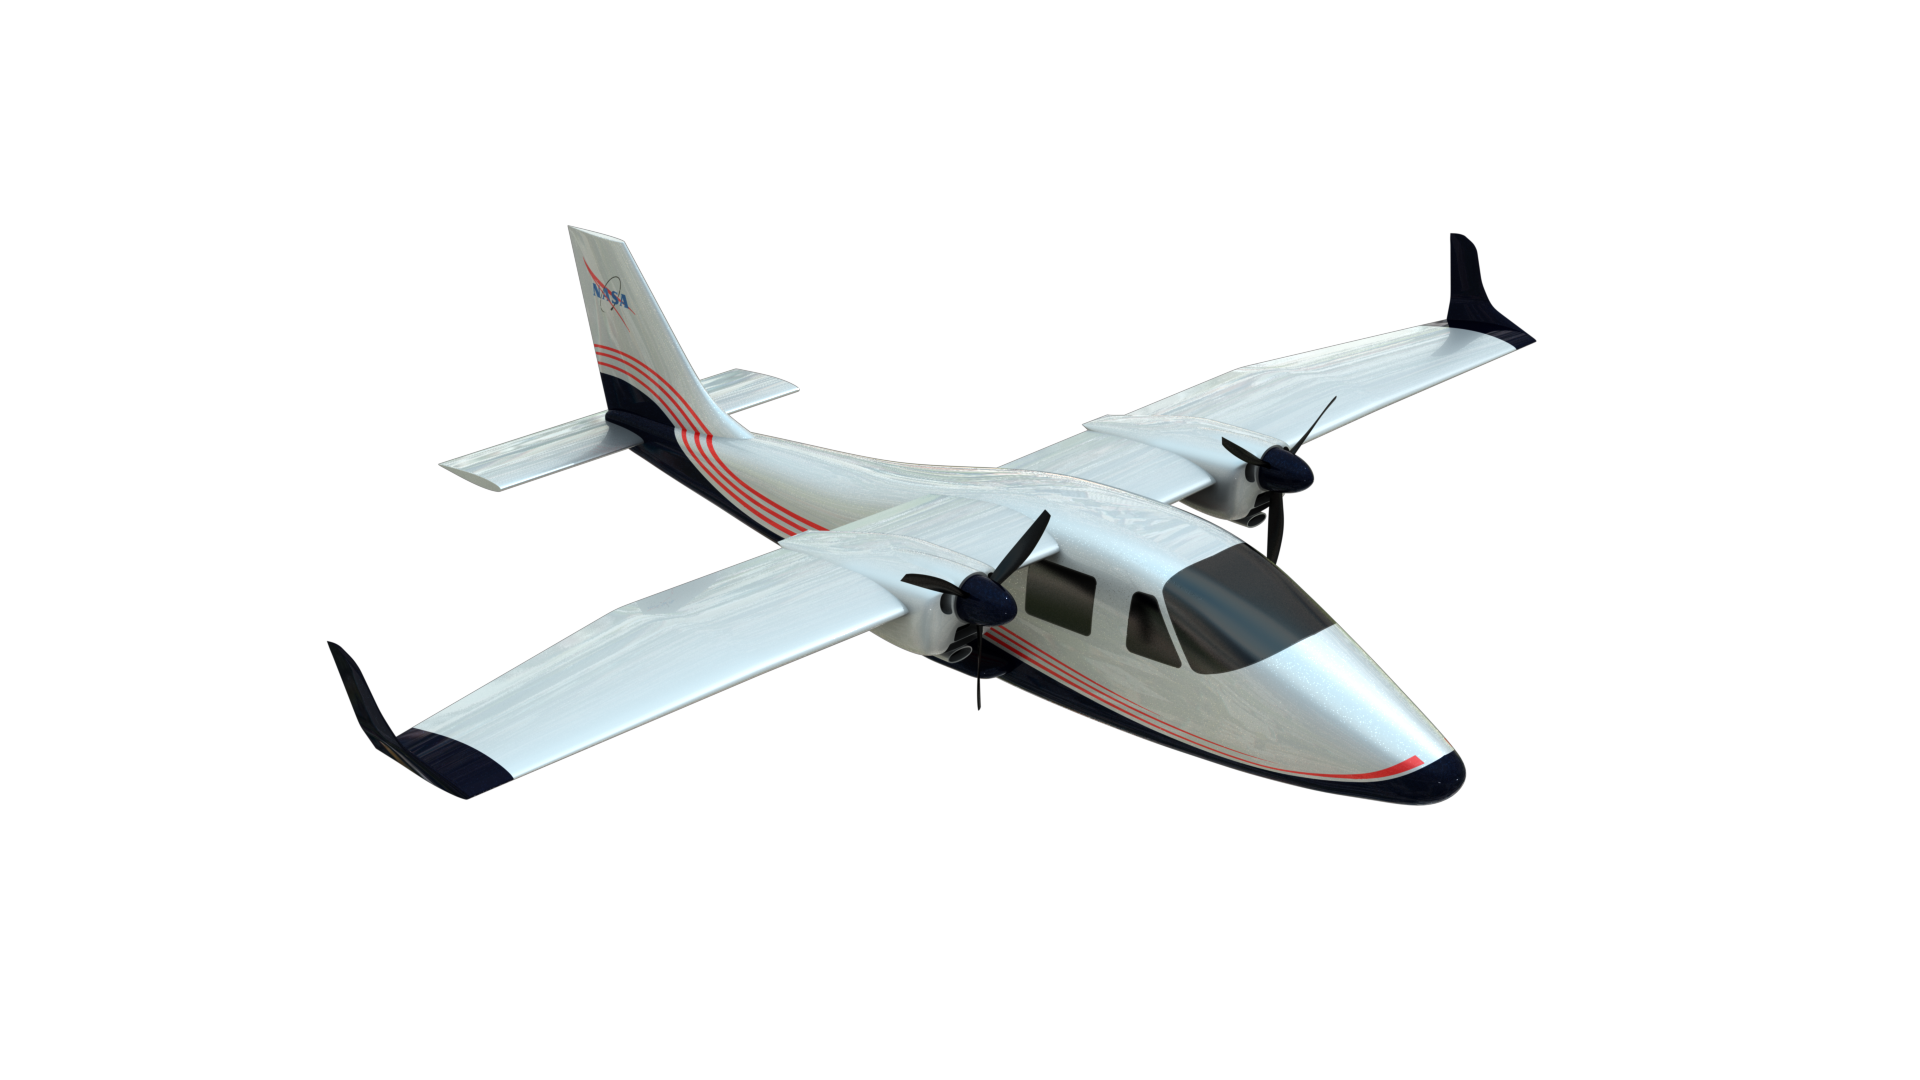
\includegraphics[width=0.5\textwidth]{figures/X57_mod2.png}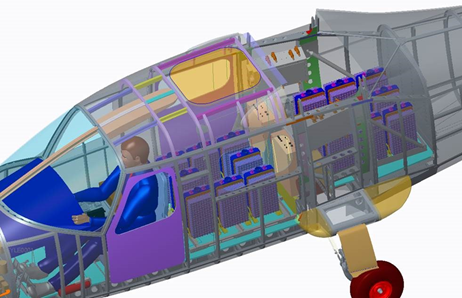
\includegraphics[width=0.5\textwidth]{figures/batt_loc.png}
	\caption{(Left) NASA's X-57 ``Maxwell'' aircraft, modification \#2 variant
	(Right) Transparent fuselage view depicting battery location and configuration into 16 battery modules}
	\label{fig:X57}
\end{figure}

Designing batteries in the context of an experimental aircraft is different than previous works on ground-based electric vehicles due to more stringent weight requirements. These requirements push the thermal design solution to be as minimal as possible, while maintaining safe operation against thermal runaway. An aircraft mission and power demand places a greater emphasis on capturing variations in OCV and internal resistance over capturing exact transient responses. Figure \ref{fig:X57} shows the X-57 Mod2 vehicle design and battery placement within the fuselage. 

\begin{table}[ht]
\begin{center}
\begin{tabular}{|l|c|c|}
\hline
 \multicolumn{1}{|c|}{\textbf{Property}} &
\multicolumn{1}{c|}{\textbf{Value}} & 
\multicolumn{1}{c|}{\textbf{Units}}\\ 
\hline
\rowcolor{LightCyan}
specific heat   & 0.83 & J/gram-\degree C \\
cell mass   & 48 & grams\\
\rowcolor{LightCyan}
discharge temp limits & -20 to 75 & \degree C \\
max discharge rate   & 15 &  Amps\\
\rowcolor{LightCyan}
max mission discharge & 9 & Amps\\
nominal voltage & 3.6 & Volts \\
\rowcolor{LightCyan}
nominal capacity & 3 & Ah\\
\hline
total pack mass & 350 & kg\\
\rowcolor{LightCyan}
pack energy density & 150 & Wh/kg\\
vehicle weight (w/o batteries) & 996 & kg\\
\rowcolor{LightCyan}
min pack voltage & 330 & Volts\\
max power draw & 120 & kW\\
\rowcolor{LightCyan}
sub-module config & 1sx20p & $\#$ of cells\\
module config & 16sx1p & $\#$ of sub-modules\\
\rowcolor{LightCyan}
pack config & 8sx2p & $\#$ of modules\\
\hline
\end{tabular}
\end{center}
\label{tab:18650batt}
\caption{X-57 Battery Properties}
\end{table}

Each battery module is comprised of 320 cylindrical 18650 cells developed by Samsung (SDI 18650-30Q) and contained within a solid block of aluminum with cores drilled for each individual cell. This solid pack body serves to contain a cell thermal runaway event by absorbing and spreading the heat sufficiently, with a central blow-off vent to release pressure gas and ejecta overboard in the event of a cell failure.

\begin{figure}[!htb]% order of placement preference: here, top, bottom
	\centering
	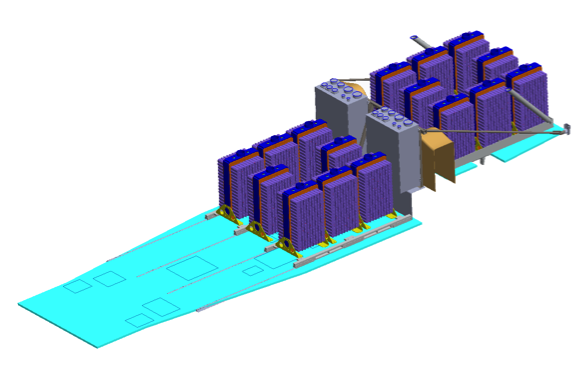
\includegraphics[width=0.7\textwidth]{figures/pallet.png}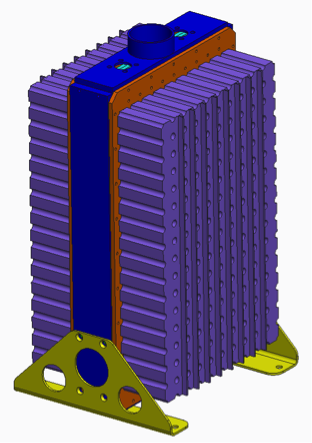
\includegraphics[width=0.25\textwidth]{figures/block.png}
	\caption{Isolated view of the battery pack and module}
	\label{fig:pallet}
\end{figure}


\section{Battery Loss Modeling} \label{BLM}

\subsection{Equivalent Circuit Model}

In order to capture transient voltage effects, non-linear capacity and thermal effects within the battery and subsequent components, a model is required to simulate battery internal resistance and voltage as a function of current draw, SOC, and battery temperature. \cite{Hu2}\textsuperscript{,} \cite{Fotouhi} 
Existing models for Lithium Ion batteries are explored in detail in multiple studies. \cite{Huria}\textsuperscript{,} \cite{Hu} These models are comprised of equivalent circuit models of varying complexity. The single RC block Thevenin model is identified as the ideal model for this application due to its simplicity and data availability, while still being able to capture transient effects and track state-of-charge within 2\% accuracy of experimental data. This model, shown in Figure \ref{fig:thevenin}, is composed of a voltage source, an internal resistance, and a parallel resistor-capacitor (RC) block to capture polarization effects. 

\begin{figure}[!htb]% order of placement preference: here, top, bottom
	\centering
	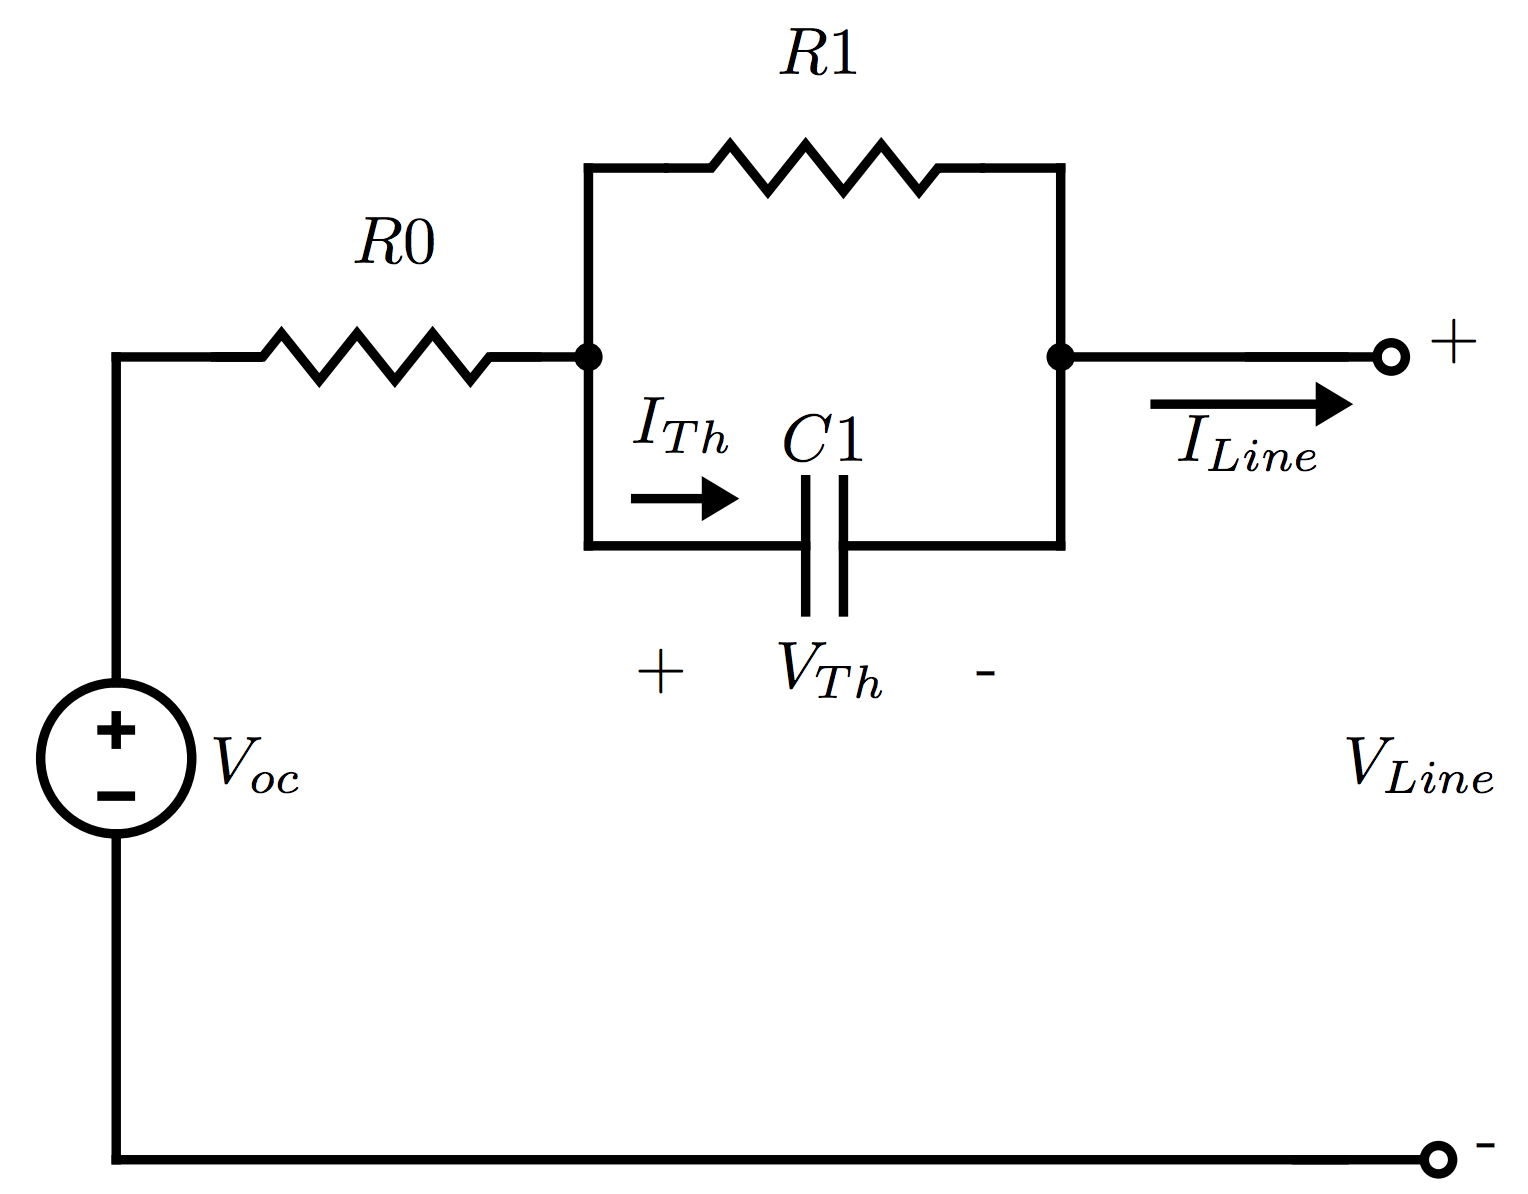
\includegraphics[width=0.5\textwidth]{figures/circuitv2.png}
	\caption{Thevenin equivalent circuit model of a battery containing a transient RC block.}
	\label{fig:thevenin}
\end{figure}

The values of each of these circuit components are interpolated from performance maps as a function of the state-of-charge, current and temperature.

\begin{align}
U_{oc},C_{Th},R_0,R_{Th} &= f(SOC, T_{batt}) \label{eq:thev1}
\end{align}
%
Subscripts $oc$, $Th$ and $L$ in Figure \ref{fig:thevenin} and Equation \ref{eq:thev1} refer to open circuit, Thevenin and line, respectively. The Thevenin voltage $U_{Th}$, battery state-of-charge $SOC$ and battery temperature $T_{batt}$ are treated as integrated states over the course of the simulation, subject to the following differential equations \cite{Hongwen}
where $Q_{max}$ is the capacity of a single cell, which is 3 $Ah$ in our model.  Each of the aircraft's two battery packs are arranged with 128 cells in series ($n_{series}$), and 40 in parallel ($n_{parallel}$).  The line voltage is computed from the open circuit and Thevenin voltage as:

\begin{align}
U_L = U_{oc} - U_{Th} - I_L R_0 \label{eq:U_L} \\
\frac{d U_{Th}}{d t} = \frac{I-\frac{U_{Th}}{R_{Th}}}{C_1}\\
\frac{d SOC}{d t} = -\frac{I}{3600*Q_{max}}
\end{align}

Note that $U_{Th}$ and $SOC$ are rates to be integrated over the mission. The electric properties of the battery pack are then:

\begin{align}
I_{pack} &= I_L \cdot n_{parallel} \label{eq:I_pack} \\
U_{pack} &= U_L \cdot n_{series} \label{eq:U_pack} \\
P_{pack} &= (I_{pack} \cdot U_{pack}) \eta_{pack} - P_{aux} \label{eq:P_pack}
\end{align}

where $\eta_{pack}$ is an efficiency knockdown to compensate for pack level losses and $P_{aux}$ accounts for auxiliary power draw.
%
The battery model is then integrated into a full aircraft model based on a demanded power driven by the overall vehicle equations of motion and propulsion models. 
A Newton solver is used to find the current load on a single cell ($I_L$) such that the power output from the battery pack is equal to the demanded power after all the efficiency knockdowns and transient responses:

\begin{align}
\mathcal{R}(I_L) &= P_{out-battery} - P_{pack} \label{eq:resid_I_L}
\end{align}
%
The battery output power is determined by reducing the requested motor input power by the efficiency losses from the wires and inverters.  Using this model, the heat output of the battery and voltage of the batteries can be accurately tracked. The battery model also dictates the current and voltage levels supplied to the other electric components, which is critical for estimating their thermal loads. The heat power generated by each cell $P_{heat}$ can be quantified, as well as the net heat load $P_{net}$ and cell temperature rise $\frac{dT}{dt}$:

\begin{align}
P_{heat} = {I_L}^2 * (R_0 + R_{Th})
\label{eq:heat}
\end{align}

\begin{align}
P_{net} = P_{heat} - \underbrace{hA(T_{batt}-T_{amb})}_{\text{convective heat out}}
\label{eq:heatBalance}
\end{align}

\begin{align}
\frac{dT}{dt} = \frac{P_{net}}{m*C_p}
\label{eq:heatRise}
\end{align}

In these equations, $h$, $m$, and $C_p$ are the heat transfer coefficient, cell mass, specific heat respectively. It's important to note that that heat capacity of the cell is impacted by the surrounding aluminum core and should be mass averaged for determining the bulk temperature rise of the entire system.


% \begin{figure}[!htb]% order of placement preference: here, top, bottom
% 	\centering
% 	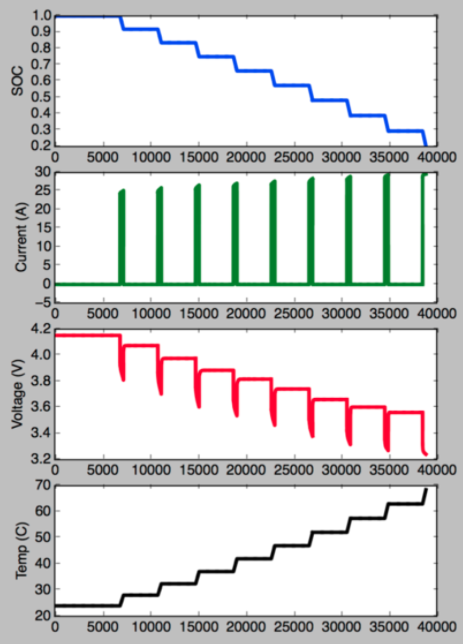
\includegraphics[width=0.5\textwidth]{figures/python.png}
% 	\caption{}
% 	\label{fig:python}
% \end{figure}

\section{Model Parameter Extraction Using Cell Characterization}

A combination of battery testing and modeling are done to distill the characteristics of the lithium ion cells that make up the battery packs into a series of performance maps. Since the Thevenin equivalent circuit variable values ($R_{0}$, $R_{Th}$, $C_{Th}$, and $U_{oc}$) are a function of state-of-charge and temperature, a series of tests are done on individual cells at different temperatures, and the data collected in these experiments are used to extract the values of open circuit voltage source ($U_{oc}$), internal resistance ($R_{0}$), and the parallel RC ($C_{Th}$, $R_{Th}$) block. The model is adaptable to different cell chemistry and configurations, assuming performance data at the cell level is available.



\subsection{Battery Cell Test Setup and Data Collection}

Cell tests were performed using an Arbin BT-2000. Data was collected every 60 seconds during rest periods, and at a rate of 2 samples/second during current pulses. Total test elapsed time, step pulse time, step index, current, voltage, discharge energy, and two temperature readings were recorded with each sample. 

\begin{figure}[!htb]% order of placement preference: here, top, bottom
	\centering
	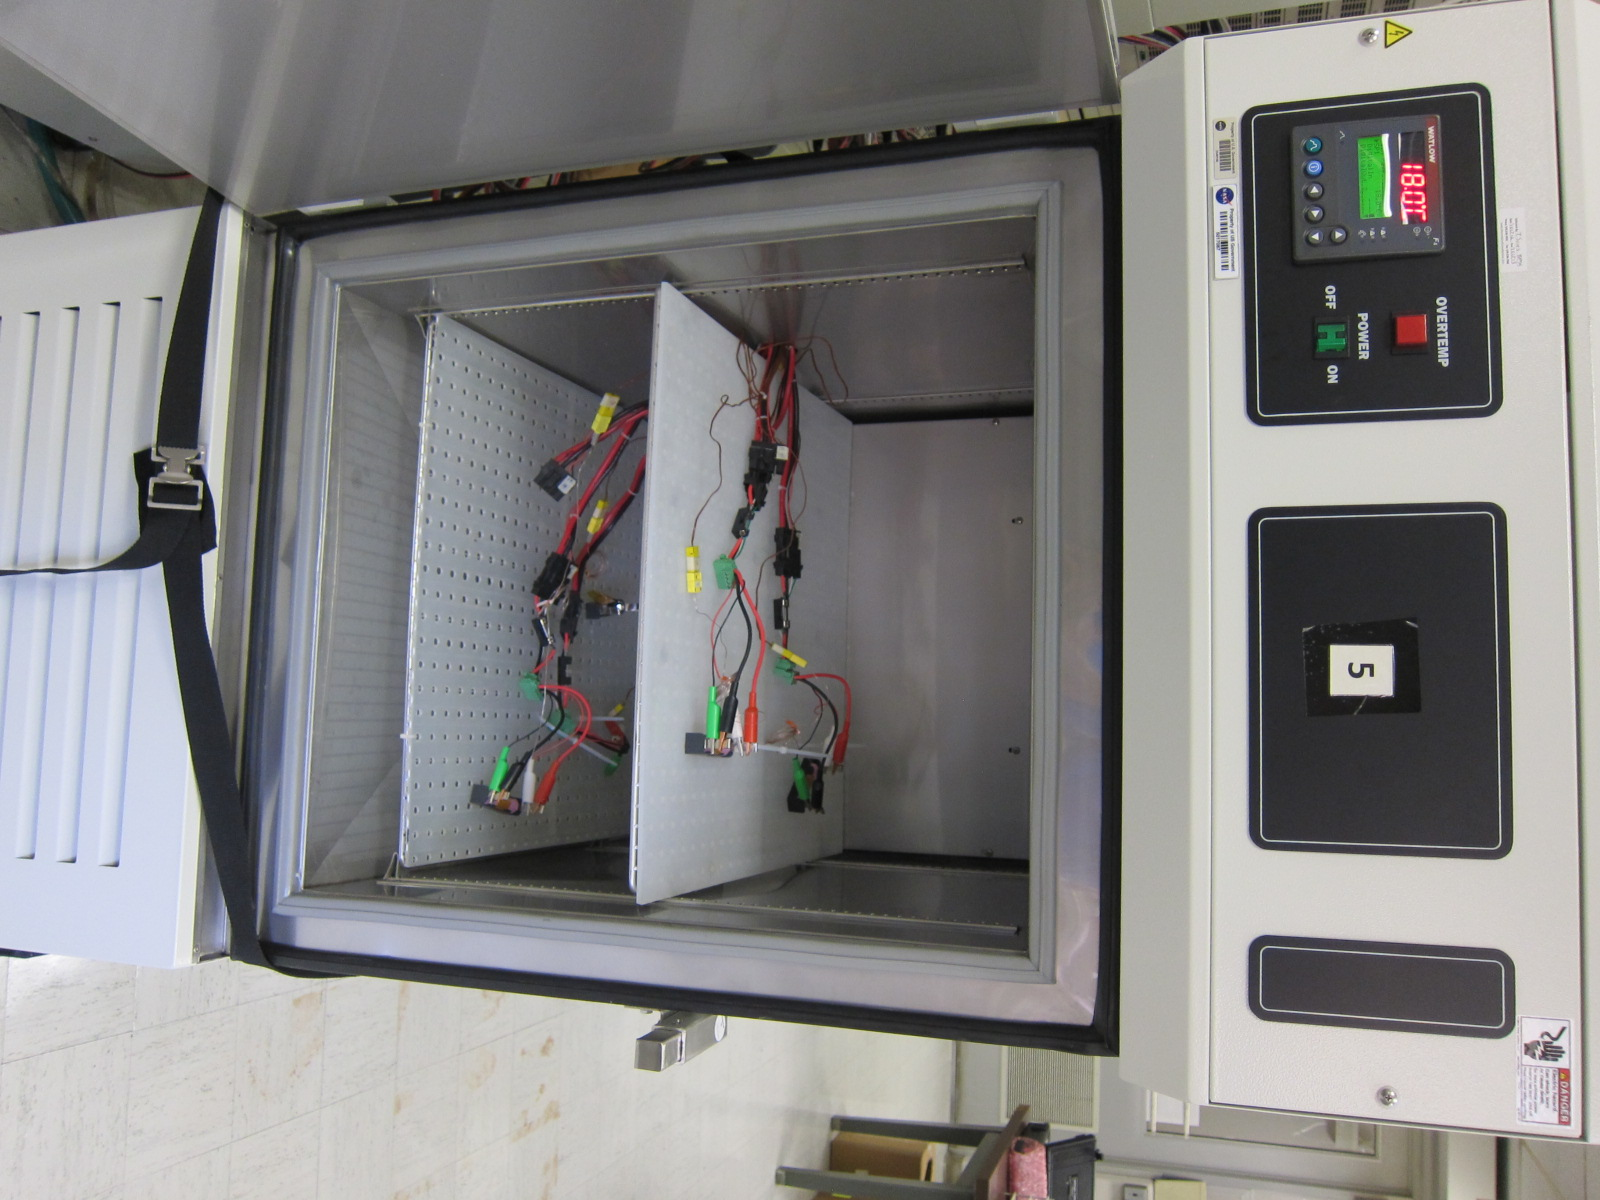
\includegraphics[width=0.5\textwidth, angle=90]{figures/ChamberFar.jpg}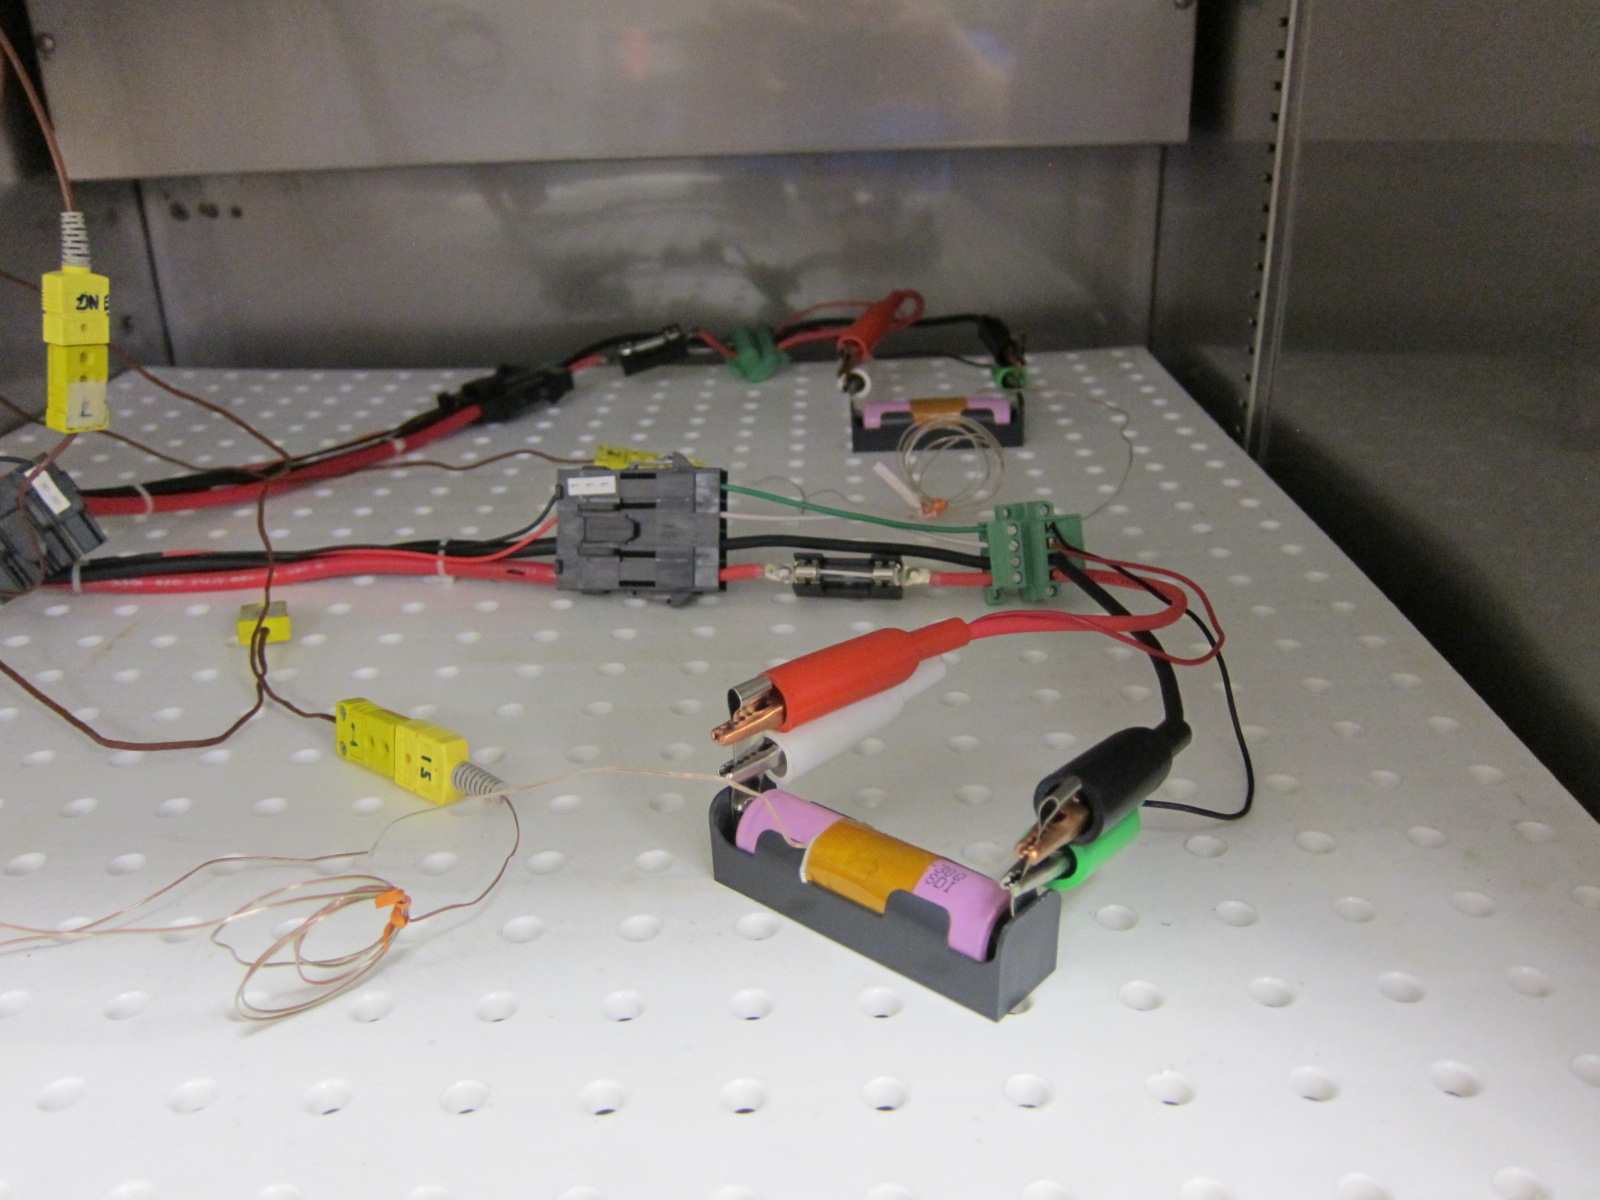
\includegraphics[width=0.5\textwidth]{figures/ChamberClose.jpg}
	\caption{Experimental battery characterization data acquisition test setup.}
	\label{fig:exp}
\end{figure}


The cells are placed in a temperature controlled chamber and outfitted with a thermocouple, as shown in Figure 4. Each temperature and discharge test combination is conducted on three lithium-ion cells. Multiple cells were tested under identical conditions to quantify variations between cells, and the 60$^\circ$C test was performed on six cells, three new cells and three previously cycled cells to compare the effects of aging. Long pauses between pulses ensured the cells remained near a constant temperature. This procedure allows equivalent circuit parameters to be fit based on the pulse transients for five different temperatures and 30 different states of charge. Each of these pulses is used to compute four battery parameters to cover all the possible battery conditions it may see during flight aboard the X-57 aircraft. 
\\
Test Procedure:
\begin{enumerate}
\item Perform cell wake-up cycles and charge:
    \begin{itemize}
        \item C/2 Charge @ 20$^\circ$C
        \item CV Taper @ 20$^\circ$C to C/20 (0.15A)
    \end{itemize}
\item Turn on temperature chamber and allow air and cells to stabilize to the specified chamber temperature for two hours. Start data acquisition.
\item  Begin discharging cells at the rates specified in the test matrix for a pulse duration of two minutes.
\item Allow cells to return to specified chamber temperature for 20 minutes.
\item If the temperature sensor shows that cell temperature increases more than 2 degrees, terminate the test.
\item Repeat steps 3-5 until batteries are discharged to three volts.
\item C/2 charge to $20\%$ SOC (0.6Ah) to stabilize cells.
\item Remove cycled cells and repeat with three fresh cells at the next temperature step in the test matrix.
\end{enumerate}

\begin{table}[ht]
\begin{center}
\begin{tabular}{|l|c|c|c|}
\hline
 \multicolumn{1}{|c|}{\textbf{Test Number}} &
 \multicolumn{1}{c|}{\textbf{Temperature}} & 
 \multicolumn{1}{c|}{\textbf{Cell Discharge Rates}} &
 \multicolumn{1}{c|}{\textbf{Cells per test}} \\ 
\hline
\rowcolor{LightCyan}
1  & 0$^\circ$C & 0.8C, 1C, 2C & 3 \\
2  & 20$^\circ$C & 0.8C, 1C, 2C & 3 \\
\rowcolor{LightCyan}
3  & 30$^\circ$C & 0.8C, 1C, 2C & 3 \\
4  & 45$^\circ$C & 0.8C, 1C, 2C & 3 \\
\rowcolor{LightCyan}
5  & 60$^\circ$C & 1C & 6 \\

\hline
\end{tabular}
\end{center}
\label{tab:battTestM}
\caption{Test Matrix}
\end{table}


\section{Parameter Extraction}

\begin{figure}[!htb]
	\centering
	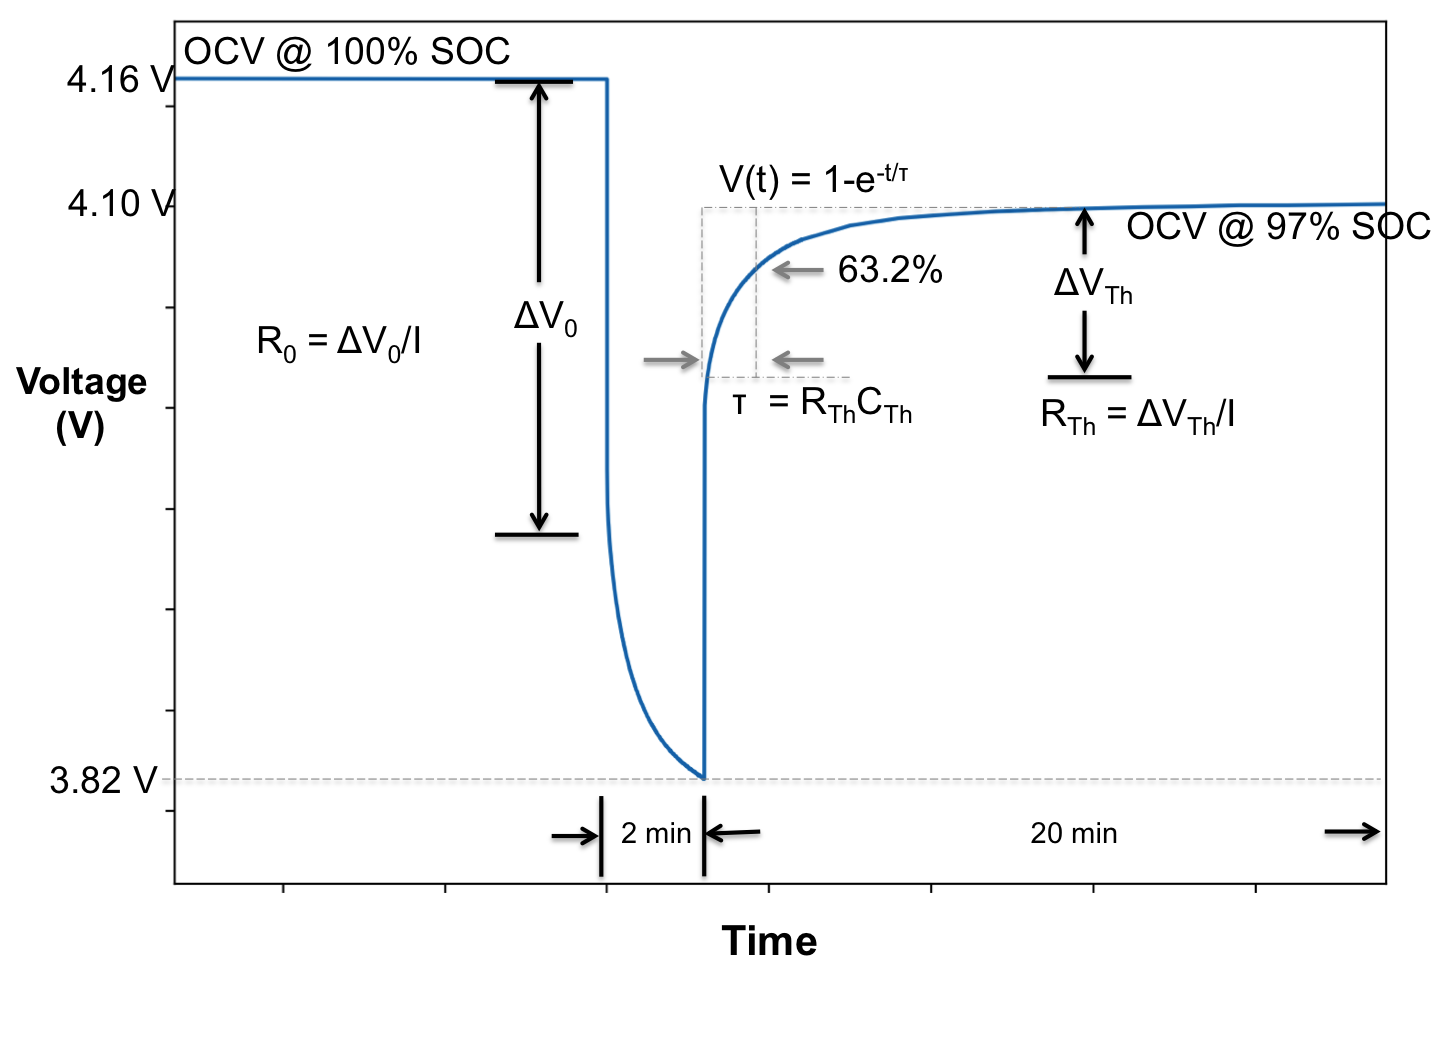
\includegraphics[width=0.75\textwidth]{figures/Batt_Char.png}
	\caption{Characterization from current pulse}
	\label{fig:BattChar}
\end{figure}

In Figure \ref{fig:BattChar} a sample voltage response is shown with annotations showing how each circuit characteristic is derived. Before each pulse, the voltage is steady at the OCV point corresponding to the SOC. During the current pulse, the voltage drops rapidly by a distance $\Delta V_{0}$ corresponding to the product of $R_{0}*I$. The subsequent logarithmic transient is then defined by the Thevenin resistance and capacitance. The non-linear return to the next OCV has a time constant equal to $R_{Th}*C_{Th}$, which is equal in magnitude to the time in seconds it takes to return 63.2\% or $(1-\frac{1}{e})$ of $\Delta V_{Th}$. This parameter extraction is repeated for every pulse corresponding to a different SOC.


\subsection{Modeling Approach to Parameter Extraction}

After the series of battery tests, the collected battery discharge data can be input into a model which uses a least squared optimization to characterize the cells, matching computes values to measured values. The experimental current discharge curve for each temperature are input into the parameter extraction model. Internal resistance ($R_{0}$), Thevenin resistance ($R_{Th}$), Thevenin capacitance ($C_{Th}$ ), and open circuit voltage ($U_{oc}$) are varied using a solver until the model computed voltage and the experimental voltage data match. The model computes each variable across the state-of-charge profile until the least squared regression minimizing the difference between experimental and computed voltages are satisfied. This computation yields a series of lookup tables which allow the battery model to interpolate $R_{0}$, $R_{Th}$, $C_{Th}$, and $U_{oc}$ as a function of battery state-of-charge and temperature. 

By separating the data into individual pulses, this process can be reduced to a linear algebra least squares problem as written:
\begin{equation}
    \begin{aligned}
        %\[
        x = 
        \begin{bmatrix}
            SOC \\
            U_{Th} \\
            U_{Th} \\
        \end{bmatrix}
        \\
        \dot{x} = Ax+bu = 
        \begin{bmatrix}
            SOC \\
            U_{1} \\
            U_{2} \\
        \end{bmatrix}
        =
        \begin{bmatrix}
            0 & 0 & 0 \\
            0 & \frac{-1}{R_{1}C_{1}} & 0 \\
           0 & 0 & \frac{-1}{R_{2}C_{2}} \\
        \end{bmatrix}
        \begin{bmatrix}
            SOC \\
            U_{1} \\
            U_{2} \\
        \end{bmatrix}
        +
        \begin{bmatrix}
            \frac{-1}{\alpha} \\
            \frac{1}{C_{1}} \\
            \frac{1}{C_{2}} \\
        \end{bmatrix}
        %\] 
    \end{aligned}
\end{equation}    

\[
y = Cx + Du = 
\begin{bmatrix}
    \alpha & -1 & -1
\end{bmatrix}
\begin{bmatrix}
    SOC \\
    U_{1} \\
    U_{2} \\
\end{bmatrix}
+
\begin{bmatrix}
    -R_{s}
\end{bmatrix}
I
\]


\begin{align}
    \tau = R_{Th}C_{Th} \\
    V_{1}(t_{charge}) = R_{1}*I_{0}*(1-e^{\frac{-t}{\tau}})\\
    V_{1}(t_{discharge}) = R_{1}*I_{0}*(1-e^{\frac{-a}{\tau}})e^{\frac{t-a}{\tau}}
\end{align}


\[
\underbrace{
\begin{bmatrix}
    y[k+1] \\
    y[k+2] \\ 
    \vdots \\
    y[k+m] \\
\end{bmatrix}
}_{\text{b}}
=
\underbrace{
\begin{bmatrix}
    y[k] & I[k] & I[k+1] \\
    y[k+1] & I[k+1] & I[k+1] \\
    \vdots  & \vdots  & \vdots \\
    y[k+m-1] & ... & I[k+m] \\
\end{bmatrix}
}_{\text{A}}
\underbrace{
\begin{bmatrix}
    \alpha_{0} \\
    b_{1} \\
    b_{2} \\
\end{bmatrix}
}_{\text{x}}
\]

\begin{align}
    A\backslash b = x
\end{align}

% \begin{figure}[!htb]
% 	\centering
% 	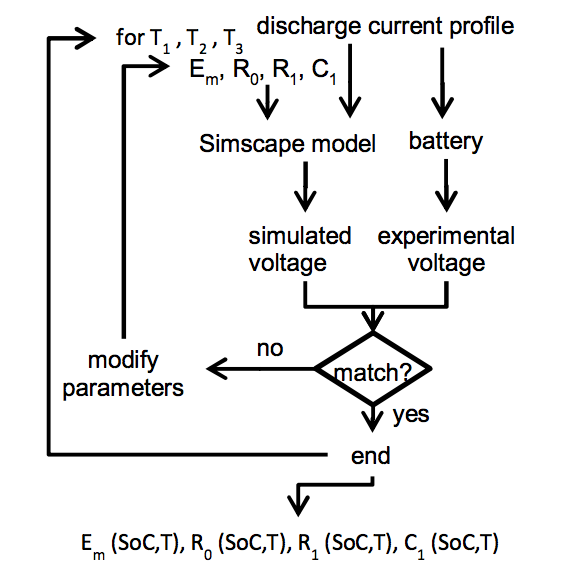
\includegraphics[width=0.5\textwidth]{figures/paramEstimation.png}
% 	\caption{Paramter Estimation Solver Loop}
% 	\label{fig:paramEst}
% \end{figure}


Depending on the current draw and temperature, the duration of each experiment is variable. Maps are calculated by creating n breakpoints to match n pulses, equally spaced from 1 to the lowest SOC. In post-processing, all maps are re-interpolated to a consistent number of breakpoints from 0 to 1. This allows a single dense 2-dimensional table to be created across a range of temperatures and charge levels.


\subsection{Results}

By creating an electrical model to mimic the cell response, it is designed to handle any arbitrary discharge current. Therefore as expected, the model performed equally well at different discharge rates. This is shown in Figure \ref{fig:paramE}, where the voltage response of two sets of experimental data and model fits are overlaid. Despite the voltages diverging between different discharge rates, the same model performed equally well on both. As a check for cell manufacturing consistency, it was also found that there was insignificant difference between cell performance exposed to the same testing conditions. Variation between temperatures is largely due to resistance.  Figure \ref{fig:AllTemp} shows experimental data for comparing cell behavior across five temperatures. The capacitance and voltage parameters did not change significantly between temperature and discharge rate tests beyond 20 $^\circ$C. 

\begin{figure}[!htb]
	\centering
	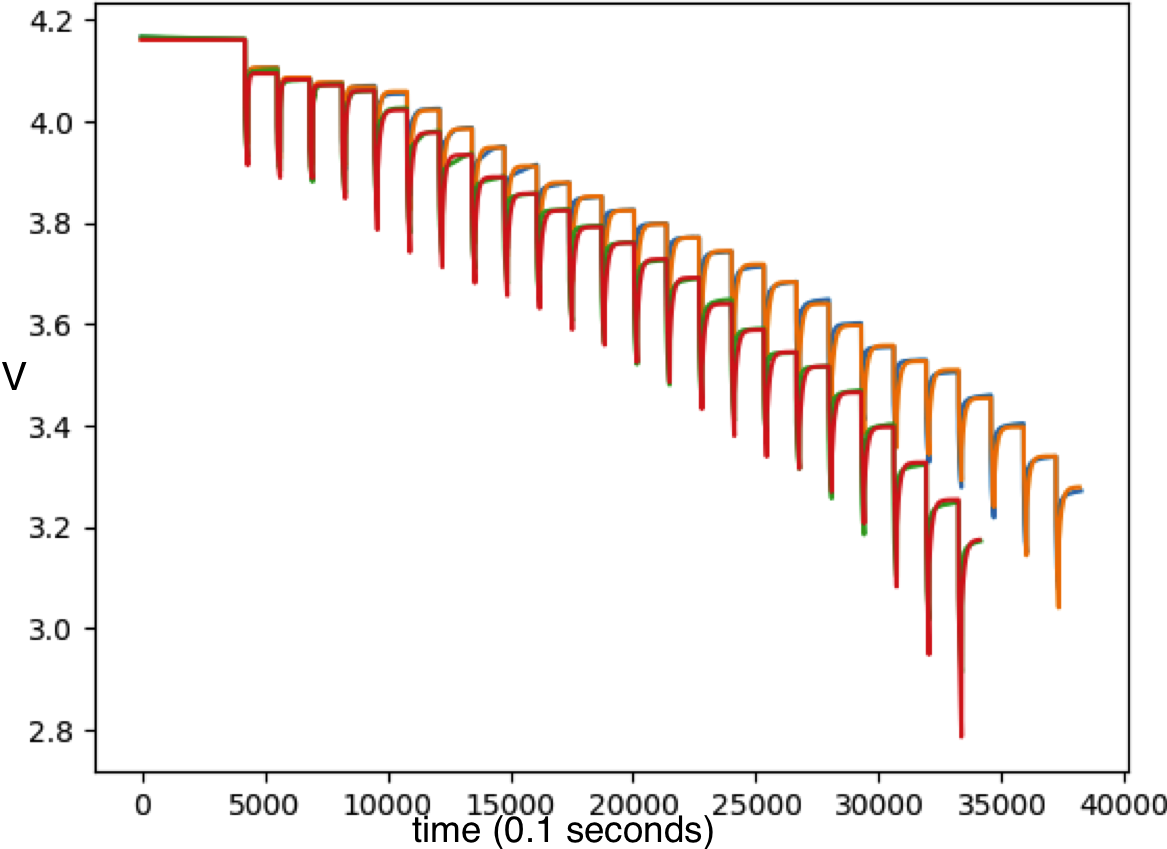
\includegraphics[width=0.75\textwidth]{figures/1_1o2C_20C_axes.png}
	%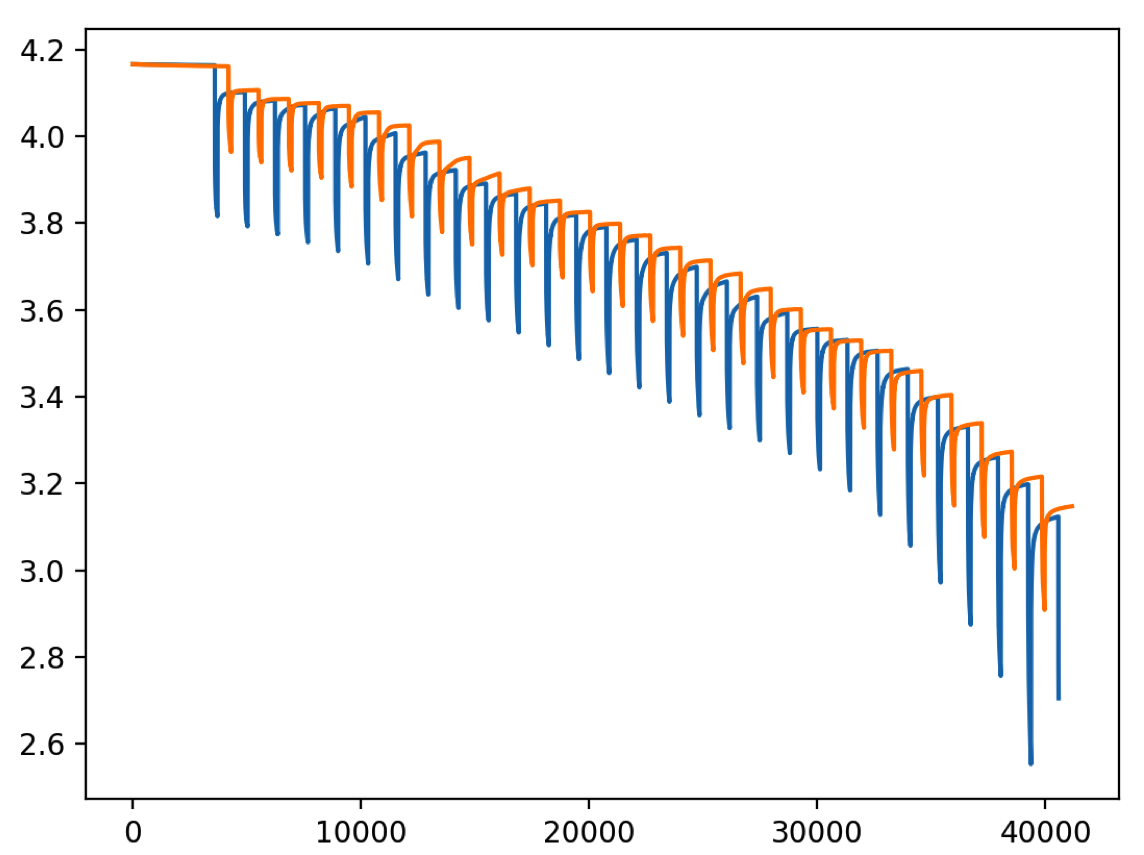
\includegraphics[width=0.5\textwidth]{figures/0_20C.png}
	\caption{Model versus test data at two different discharge rates. Red - 1.2C model vs Green - 1.2C test data, Orange 1C model vs Blue 1C test data, shows the same model working regardless of discharge rate.}
	\label{fig:paramE}
\end{figure}

\begin{figure}[!htb]
	\centering
	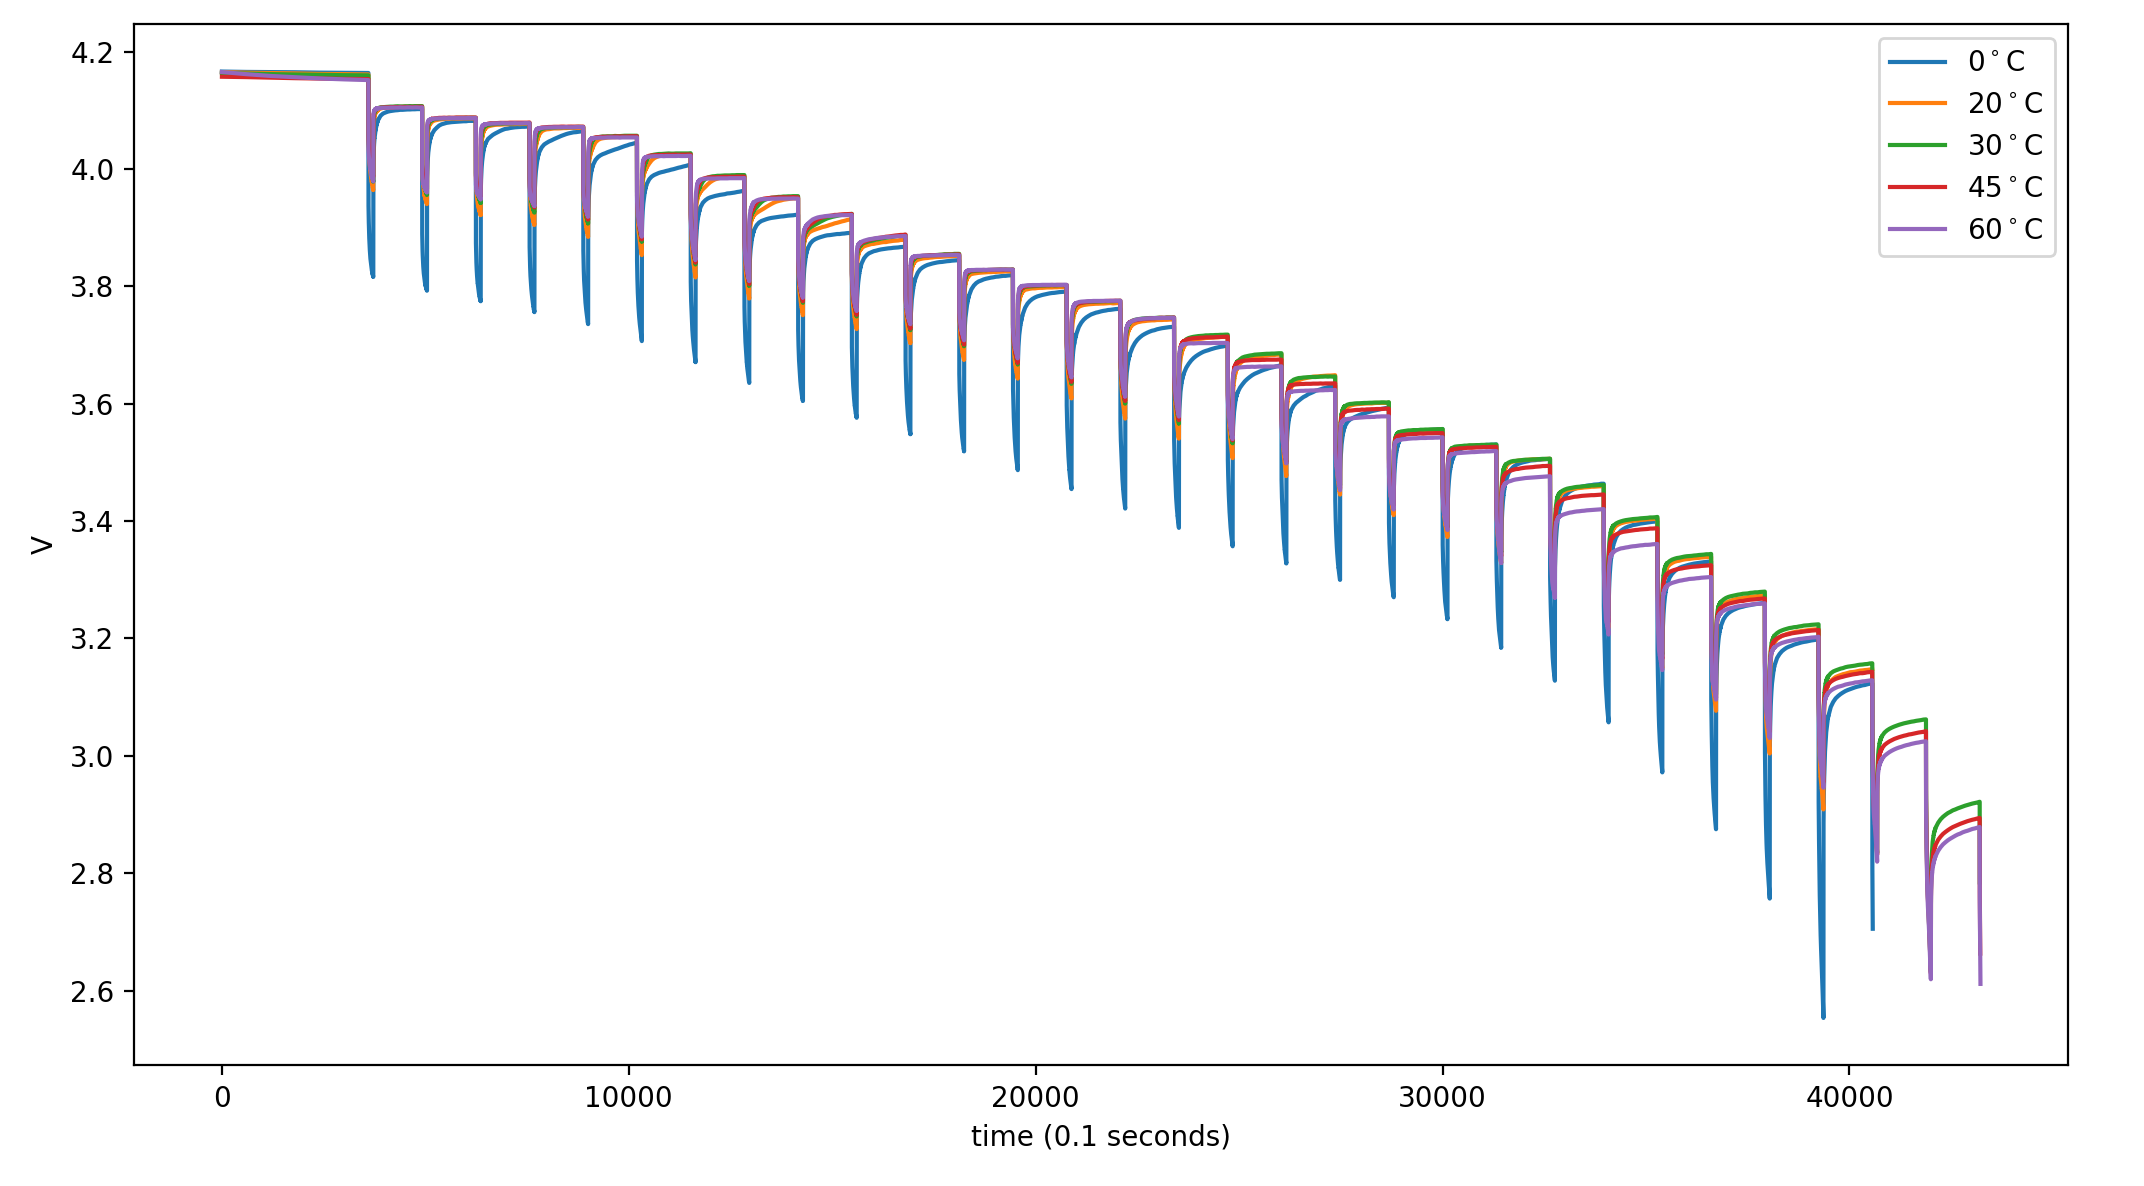
\includegraphics[width=1.0\textwidth]{figures/All_Temp.png}
	\caption{Battery voltage response to current pulses across five temperatures}
	\label{fig:AllTemp}
\end{figure}


% JSG: This paragraph is confusing, because it sounds like you have some data on aging that you'll present...so I changed wording a bit. You deal with this in a later section. I think you can just skip this part
% The aging of the cells is generally known to have a noticeable effect on voltage levels at lower SOC as depicted below, bu However, experimentally validating the aging model is beyond the scope of this study.

Figure \ref{fig:Map} shows the variation of each parameter across 4 temperatures and a series of SOCs. Capacitance is not shown, since it wasn't shown to have significant variant across temperature or charge. This parameter can stay at a value of 2000. The open-circuit voltage decreases with reduced SOC, and it should be noted that this curve is not expected to match battery manufacturer performance curves. These curves are reproduced with the model in Figure \ref{fig:curve}. Thevenin resistance follows a slow upward trend with decreasing charge, with a noticeable jump in resistance for colder temperatures. $R_0$ also increases substantially at 0$^\circ$C, but remains flat until very low SOC.

\begin{figure}[!htb]
	\centering
	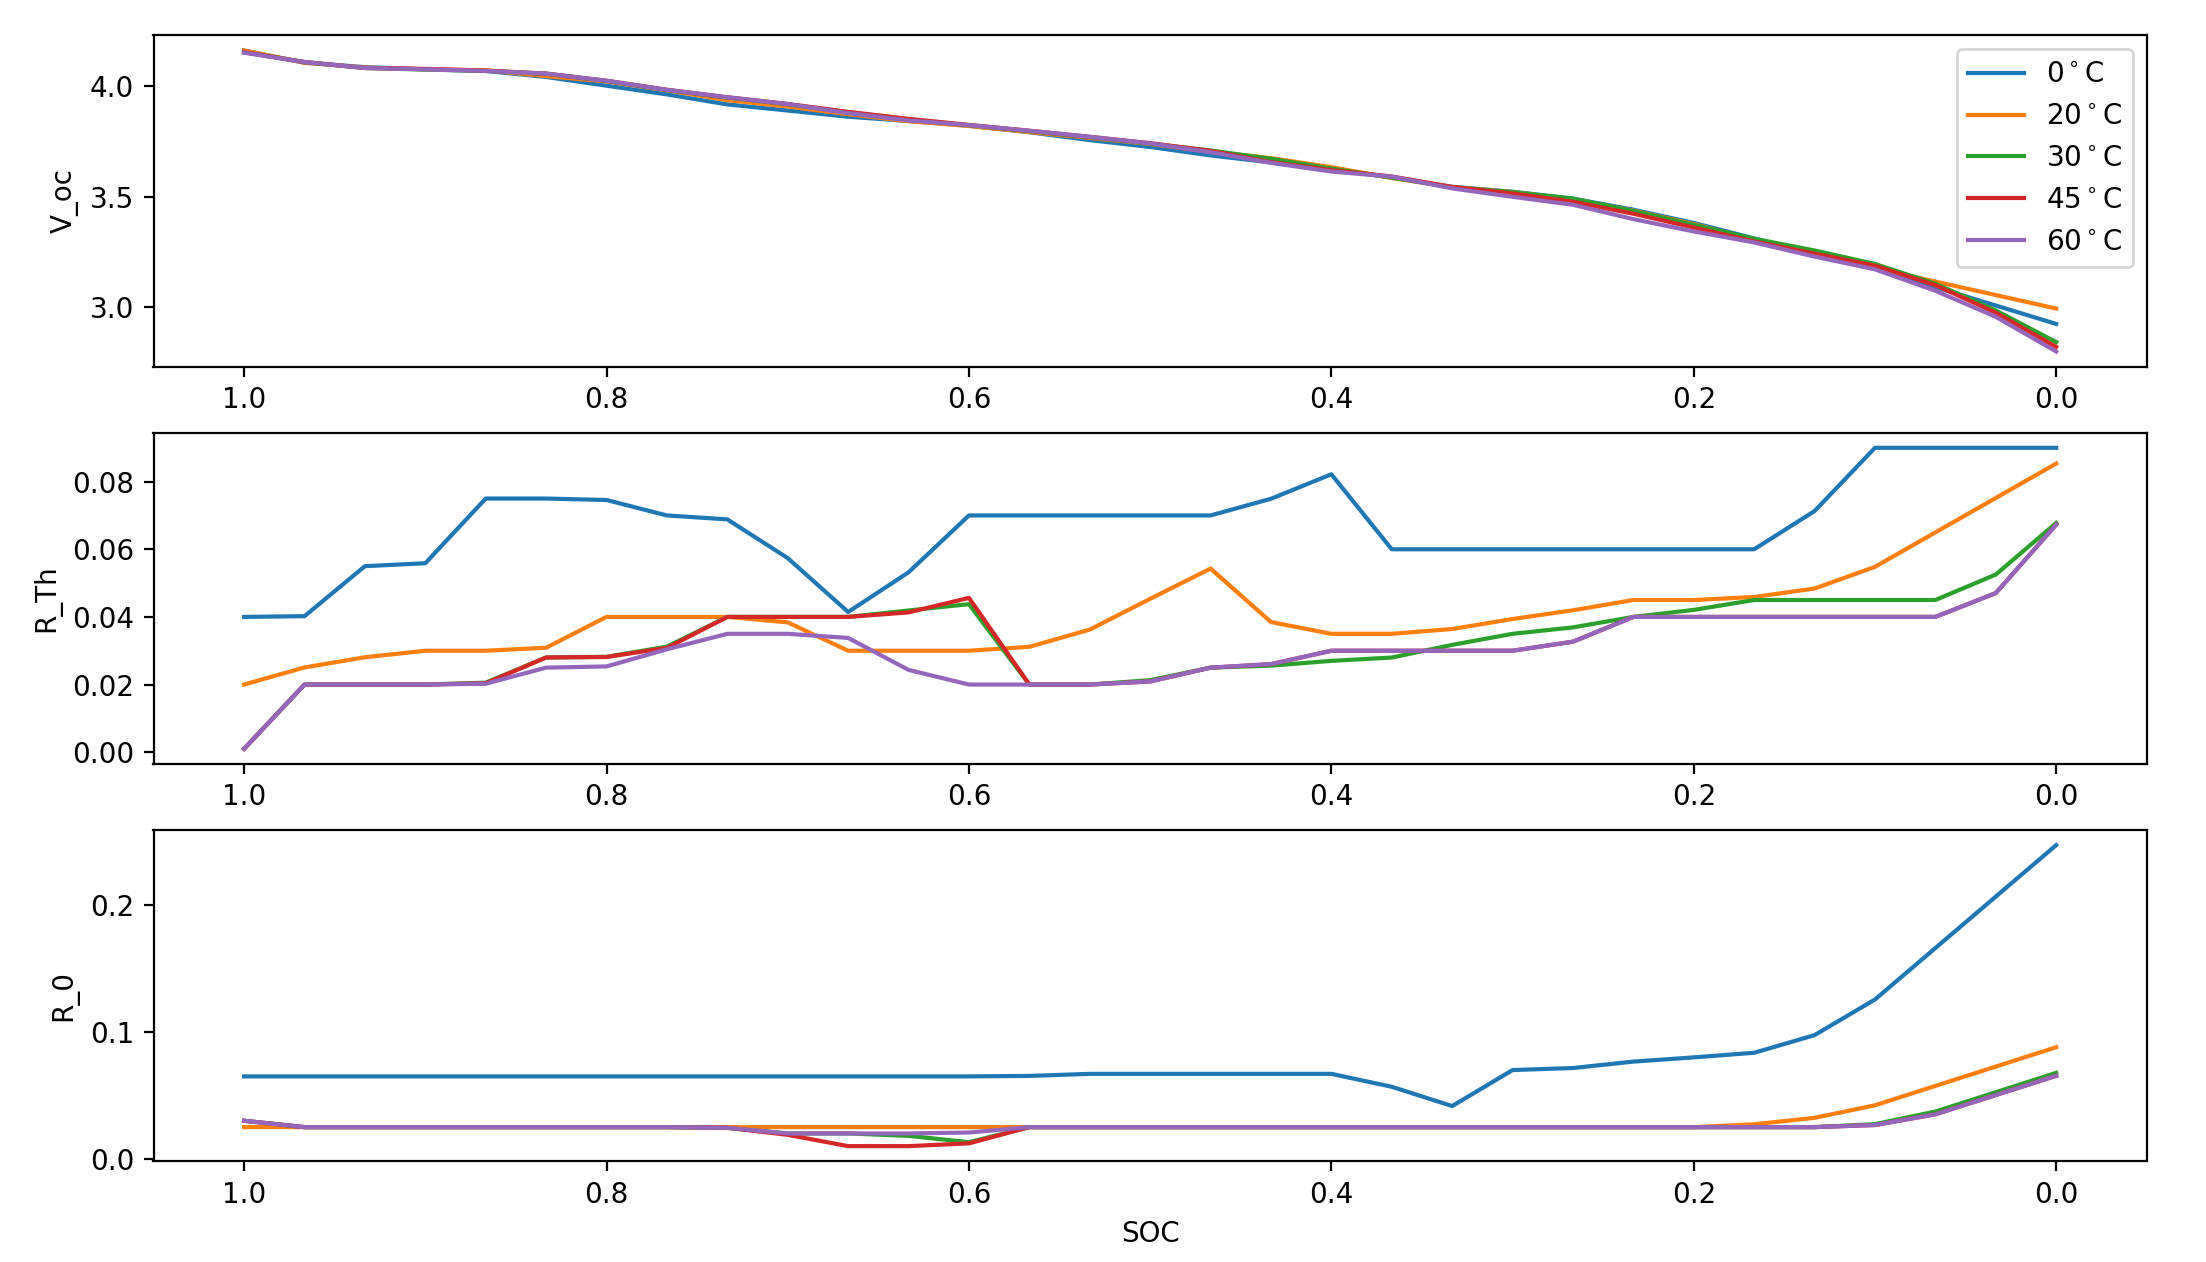
\includegraphics[width=1.0\textwidth]{figures/maps.png}
	\caption{Parameter variation with temperature and SOC}
	\label{fig:Map}
\end{figure}


\begin{figure}[!htb]
	\centering
	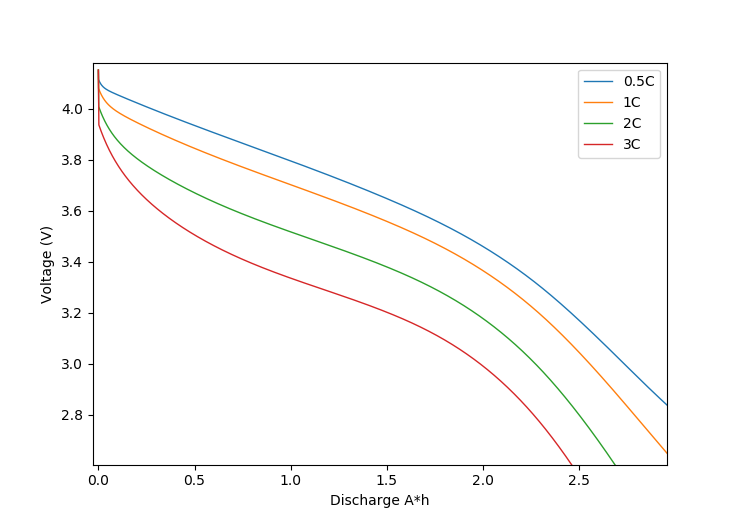
\includegraphics[width=0.75\textwidth]{figures/curve.png}
	\caption{Replication of standard manufacturer performance curve}
	\label{fig:curve}
\end{figure}

Figure \ref{fig:curve} shows the battery model used to simulate a standard cell manufacturer performance curve over a steady discharge rate. Shown in Figure \ref{fig:L1_004} is the battery response to a nominal flight profile compared to the model. The top graph shows test voltage data in blue, and the prediction model in orange. The bottom graph shows the same profile but shows predicted temperature. A green line is also plotted to show temperature estimates assuming a constant loss rate of 8 percent. As expected, assuming a constant efficiency over-estimates the initial losses at high states of charge and under-estimates the losses at low states of charge. This highlights the benefit of the model in capturing non-linear resistances to accurately track temperature.

\begin{figure}[!htb]
	\centering
	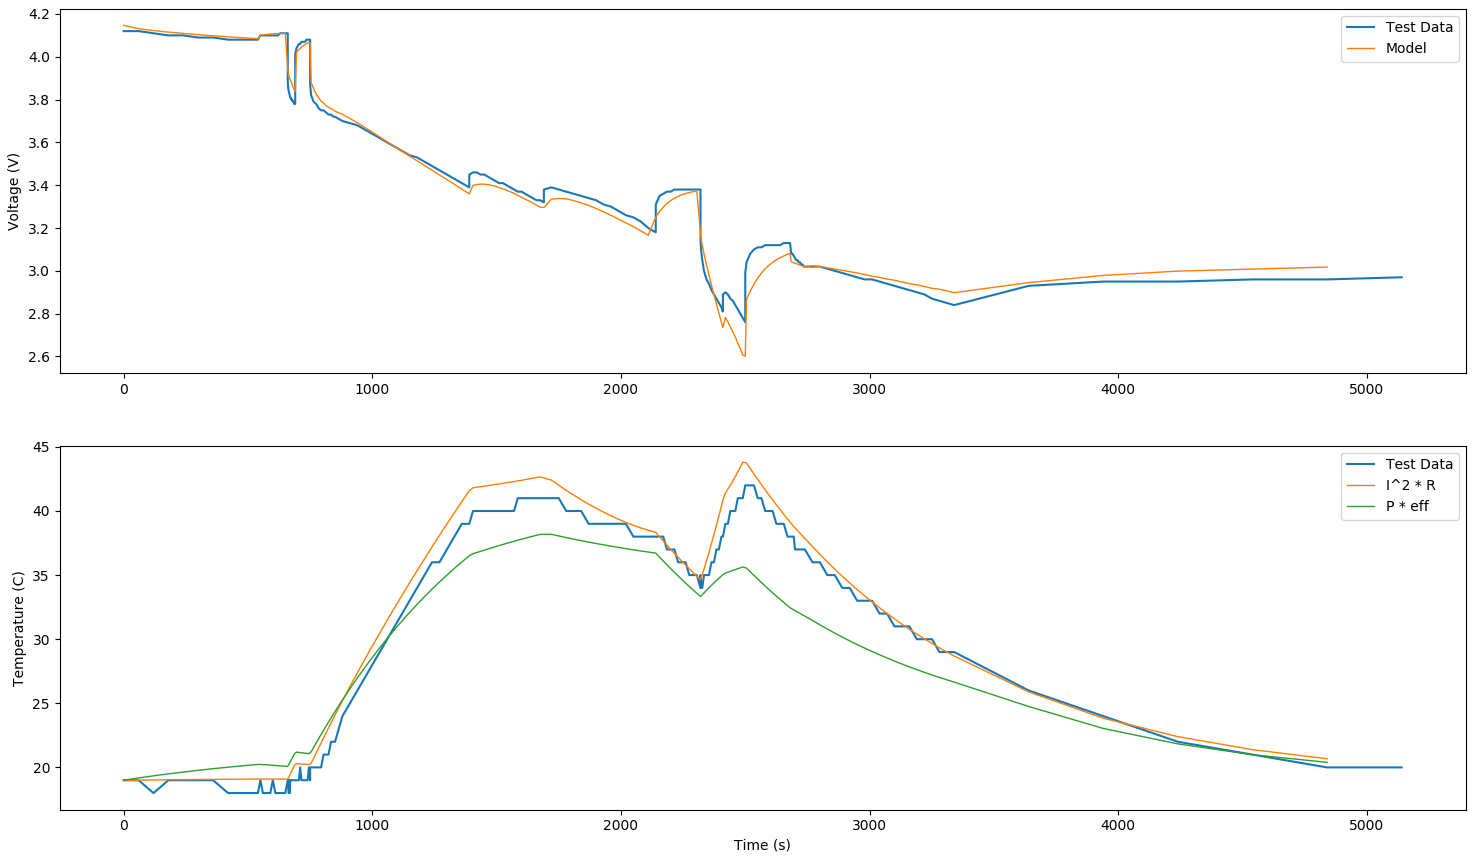
\includegraphics[width=1.0\textwidth]{figures/x57_L1_004.png}
	\caption{Model performance against a nominal flight profile}
	\label{fig:L1_004}
\end{figure}

Applying these new battery characteristics to a full vehicle model of X-57 resulted in a decrease in expected vehicle performance over the previously assumed prismatic cell data. The notional mission profile shown below depicts the reduction in cruise time of the vehicle. 

\begin{figure}[!htb]
	\centering
	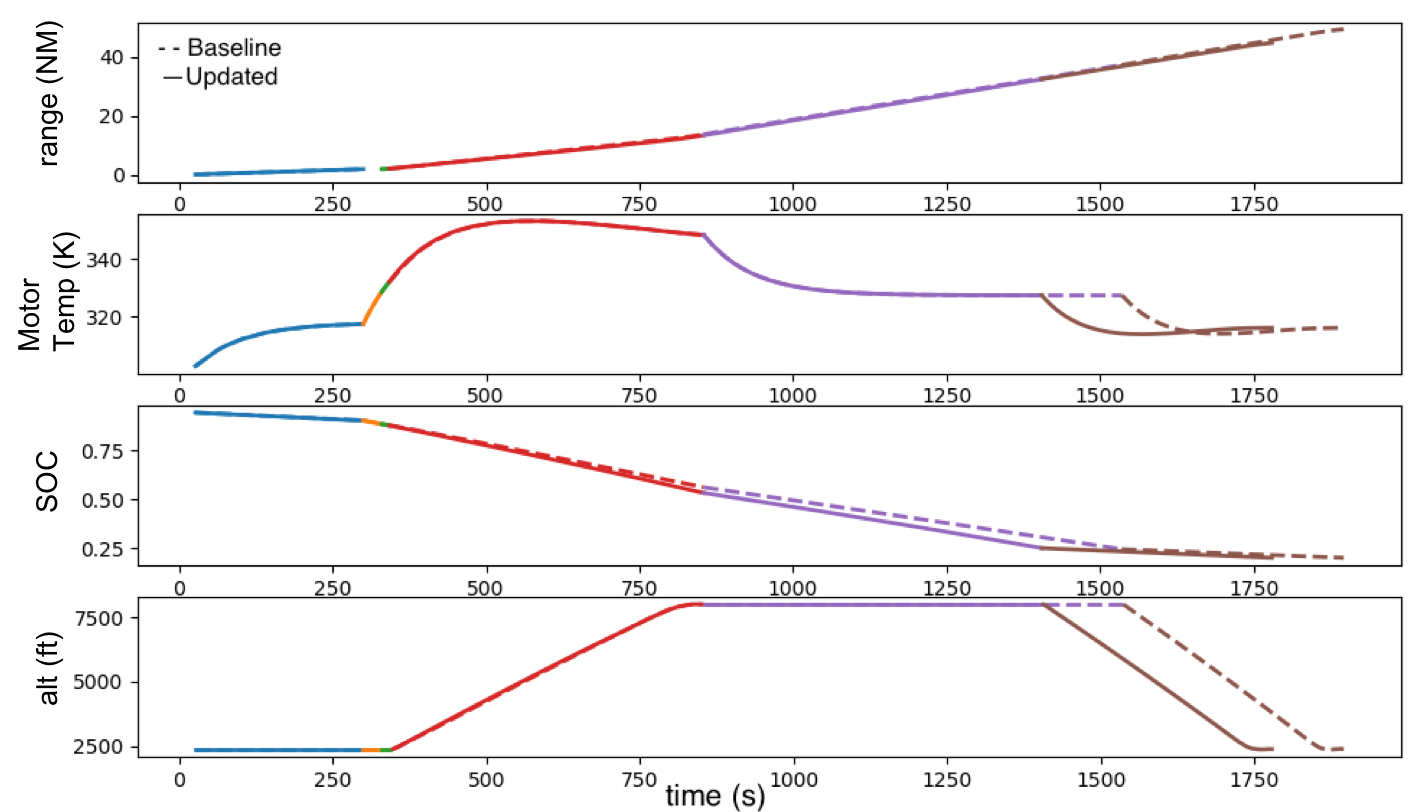
\includegraphics[width=1.0\textwidth]{figures/batt_mission_axes2.png}
	\caption{Impact in performance at the vehicle level, compared to baseline maps. Each color represents a different mission segment. Taxi, motor check, climb, cruise, and descent respectively from left to right.}
	\label{fig:Mission}
\end{figure}

\section{Model Limitations}
The model does not currently account for capacity fade and aging due to high discharge rates or repeated cycles. Modifiers could be added to the model \cite{Ning}, however it was deemed unnecessary for X-57 which will only be flown a very limited number of times. Given the limited test points, the model is not well fit to experimental data at states of charge below 20 percent where the behavior becomes more divergent. This limitation is deemed acceptable given that the vehicle must avoid fully draining the battery to avoid permanent capacity fade. As discussed in section \ref{BLM}, there are numerous higher fidelity battery modeling techniques, and this method was chosen for its simplicity and speed.


\section{Conclusions and Future Work}

Various figures of merit were used to compare a purely mathematical battery modeling method to a combined electrical and analytical model. The parameters necessary for the equivalent circuit model were experimentally derived using the described test procedures and optimization routine. The error in each type of model was quantified for a range of transient profiles and operating temperatures. The purely analytical model provides a more generic tool set, that can be more readily defined using manufacturer's specification data. The electrical model is able to capture a higher degree of transient behavior over a range of charge levels, which becomes increasingly critical for transients involving many throttle changes. Both methods can be used interchangeably as the basis for pack level calculations and vehicle level models, depending on the designer's needs.


\section{Acknowledgements}

The authors would like to thank the rest of the X-57 team, the battery team, and the Electric Power Systems for their collaboration. Additional thanks to the NASA Flight Demonstration and Capabilities Project for sponsoring this work.

% produces the bibliography section when processed by BibTeX

\bibliography{bibtex_database}
\bibliographystyle{aiaa}

\pagebreak
The raw data can be found at:\\
\url{https://github.com/jcchin/Battery-Performance-Modeling-on-Maxwell-X_57/blob/master/Data.zip}

The code repository can be found at:\\
\url{https://github.com/jcchin/Battery-Performance-Modeling-on-Maxwell-X_57/tree/master/code}
\subsection{Battery Performance Maps}
\setminted{fontsize=\tiny,baselinestretch=1}
\begin{minted}{python}

battery.T_bp = np.array([0., 20., 30., 45.])
battery.SOC_bp = np.array( [0.        , 0.03333333, 0.06666667, 0.1       , 0.13333333, 0.16666667,
 0.2       , 0.23333333, 0.26666667, 0.3       , 0.33333333, 0.36666667,
 0.4       , 0.43333333, 0.46666667, 0.5       , 0.53333333, 0.56666667,
 0.6       , 0.63333333, 0.66666667, 0.7       , 0.73333333, 0.76666667,
 0.8       , 0.83333333, 0.86666667, 0.9       , 0.93333333, 0.96666667,
 1.        ] )
battery.tU_oc = np.array([ [2.92334783,3.00653623,3.08972464,3.17291304,3.23989855,3.31010145,
 3.3803913 ,3.44033333,3.49033333,3.52169565,3.54391304,3.58695652,
 3.62095652,3.65437681,3.68604348,3.72430435,3.75531884,3.79102899,
 3.82030435,3.84181159,3.86124638,3.88921739,3.91686957,3.96223188,
 4.00169565,4.04117391,4.06849275,4.07573913,4.08571014,4.10571014,
 4.161     ] ,  [2.99293893,3.05400763,3.11507634,3.17614504,3.23506616,3.30371247,
 3.37521374,3.43605852,3.48697455,3.5200229 ,3.54251908,3.58374046,
 3.6329313 ,3.67379644,3.70287532,3.73784733,3.76526463,3.79174809,
 3.81922901,3.84108142,3.87212214,3.90738931,3.93615267,3.98113995,
 4.02093893,4.04504071,4.07114758,4.07583969,4.08371501,4.10560814,
 4.161     ] ,  [2.84084639,2.98428484,3.1050295 ,3.19464496,3.25566531,3.309059  ,
 3.37185148,3.43473652,3.49059613,3.51955239,3.541353  ,3.58558494,
 3.62641607,3.6708881 ,3.70814547,3.7392177 ,3.76822075,3.79592981,
 3.82260427,3.84986368,3.88146592,3.91739674,3.94798779,3.98188403,
 4.02274568,4.05623296,4.06830824,4.07468871,4.08175788,4.10853306,
 4.153     ] ,  [2.81925101,2.97410931,3.09861134,3.18674899,3.24142105,3.29678138,
 3.35963563,3.42195951,3.47637247,3.51383806,3.54319838,3.59076923,
 3.61940891,3.65574089,3.7067004 ,3.74153441,3.77023887,3.79773684,
 3.82421053,3.85139271,3.88311336,3.91906478,3.94918219,3.98310931,
 4.02401215,4.05611741,4.07036842,4.07774494,4.08190283,4.10867206,
 4.153     ] ])
battery.tC_Th = np.array([ [2000.,2000.,2000.,2000.,2000.,2000.,2000.,2000.,2000.,2000.,2000.,2000.,
 2000.,2000.,2000.,2000.,2000.,2000.,2000.,2000.,2000.,2000.,2000.,2000.,
 2000.,2000.,2000.,2000.,2000.,2000.,2000.] ,  [2000.,2000.,2000.,2000.,2000.,2000.,2000.,2000.,2000.,2000.,2000.,2000.,
 2000.,2000.,2000.,2000.,2000.,2000.,2000.,2000.,2000.,2000.,2000.,2000.,
 2000.,2000.,2000.,2000.,2000.,2000.,2000.] ,  [2000.,2000.,2000.,2000.,2000.,2000.,2000.,2000.,2000.,2000.,2000.,2000.,
 2000.,2000.,2000.,2000.,2000.,2000.,2000.,2000.,2000.,2000.,2000.,2000.,
 2000.,2000.,2000.,2000.,2000.,2000.,2000.] ,  [2000.,2000.,2000.,2000.,2000.,2000.,2000.,2000.,2000.,2000.,2000.,2000.,
 2000.,2000.,2000.,2000.,2000.,2000.,2000.,2000.,2000.,2000.,2000.,2000.,
 2000.,2000.,2000.,2000.,2000.,2000.,2000.] ])
battery.tR_Th = np.array([ [0.09      ,0.09      ,0.09      ,0.09      ,0.07130435,0.06      ,
 0.06      ,0.06      ,0.06      ,0.06      ,0.06      ,0.06      ,
 0.08217391,0.07492754,0.07      ,0.07      ,0.07      ,0.07      ,
 0.07      ,0.05318841,0.04144928,0.0573913 ,0.06884058,0.07      ,
 0.07456522,0.075     ,0.075     ,0.05586957,0.055     ,0.04021739,
 0.04      ] ,  [0.08534351,0.07516539,0.06498728,0.05480916,0.04838931,0.04589059,
 0.045     ,0.045     ,0.04195929,0.03937405,0.03642494,0.035     ,
 0.035     ,0.03848601,0.05430025,0.04534351,0.03624682,0.03115776,
 0.03      ,0.03      ,0.03      ,0.03839695,0.04      ,0.04      ,
 0.04      ,0.03089059,0.03      ,0.03      ,0.02807125,0.02505344,
 0.02      ] ,  [0.0677823 ,0.05252289,0.045     ,0.045     ,0.045     ,0.045     ,
 0.04207528,0.04      ,0.03690234,0.035     ,0.0317294 ,0.02798576,
 0.027     ,0.025588  ,0.025     ,0.02129705,0.02      ,0.02      ,
 0.04377416,0.04190234,0.04      ,0.04      ,0.04      ,0.03121058,
 0.02820753,0.028     ,0.02055341,0.02      ,0.02      ,0.02      ,
 0.001     ] ,  [0.06728745,0.04704453,0.04      ,0.04      ,0.04      ,0.04      ,
 0.04      ,0.04      ,0.03267206,0.03      ,0.03      ,0.03      ,
 0.03      ,0.02603239,0.025     ,0.02091093,0.02      ,0.02      ,
 0.04562753,0.04133603,0.04      ,0.04      ,0.04      ,0.0308502 ,
 0.02814575,0.028     ,0.02038866,0.02      ,0.02      ,0.02      ,
 0.001     ] ])
battery.tR_0 = np.array([ [0.2473913 ,0.20681159,0.16623188,0.12565217,0.09753623,0.08362319,
 0.08      ,0.07666667,0.0715942 ,0.07      ,0.0415942 ,0.05681159,
 0.067     ,0.067     ,0.067     ,0.067     ,0.067     ,0.06537681,
 0.065     ,0.065     ,0.065     ,0.065     ,0.065     ,0.065     ,
 0.065     ,0.065     ,0.065     ,0.065     ,0.065     ,0.065     ,
 0.065     ] ,  [0.08801527,0.07274809,0.05748092,0.04221374,0.03231552,0.02722646,
 0.025     ,0.025     ,0.025     ,0.025     ,0.025     ,0.025     ,
 0.025     ,0.025     ,0.025     ,0.025     ,0.025     ,0.025     ,
 0.025     ,0.025     ,0.025     ,0.025     ,0.025     ,0.025     ,
 0.025     ,0.025     ,0.025     ,0.025     ,0.025     ,0.025     ,
 0.025     ] ,  [0.0677823 ,0.05252289,0.03726348,0.02733469,0.025     ,0.025     ,
 0.025     ,0.025     ,0.025     ,0.025     ,0.025     ,0.025     ,
 0.025     ,0.025     ,0.025     ,0.025     ,0.025     ,0.025     ,
 0.01311292,0.01809766,0.02      ,0.02      ,0.02430824,0.025     ,
 0.025     ,0.025     ,0.025     ,0.025     ,0.025     ,0.025     ,
 0.03      ] ,  [0.06546559,0.0502834 ,0.03510121,0.02663968,0.025     ,0.025     ,
 0.025     ,0.025     ,0.025     ,0.025     ,0.025     ,0.025     ,
 0.025     ,0.025     ,0.025     ,0.025     ,0.025     ,0.025     ,
 0.01218623,0.01      ,0.01      ,0.01890688,0.02451417,0.025     ,
 0.025     ,0.025     ,0.025     ,0.025     ,0.025     ,0.025     ,
 0.03      ] ])
 
 \end{minted}

\begin{figure}[!htb]
	\centering
	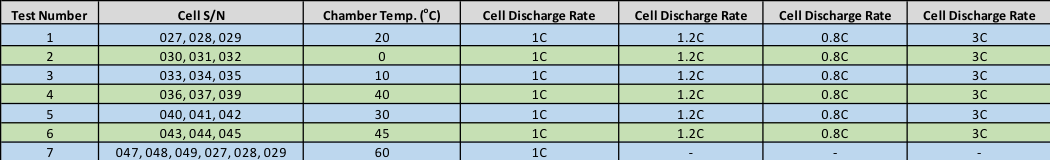
\includegraphics[width=1.0\textwidth]{figures/Test_Matrix.png}
	\caption{Test Matrix}
	\label{fig:TestMatrix}
\end{figure}

\begin{figure}[!htb]
	\centering
	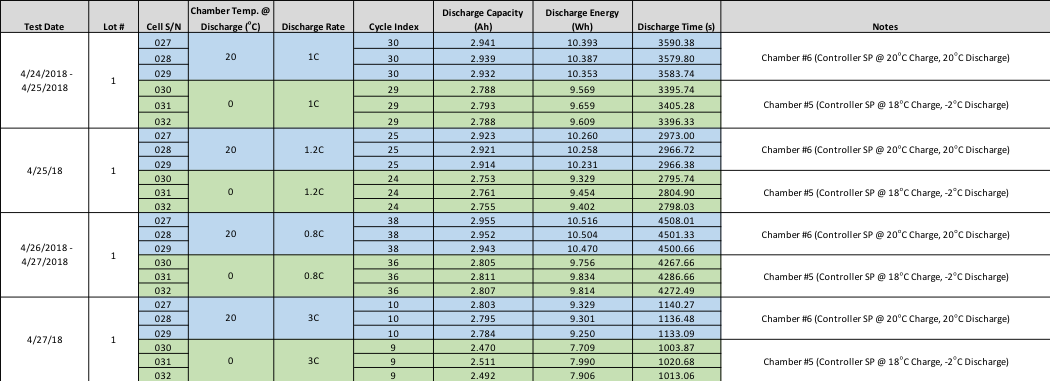
\includegraphics[width=1.0\textwidth]{figures/Test1Summary.png}
	\caption{Test 1 Summary}
	\label{fig:Test1Summary}
\end{figure}

\begin{figure}[!htb]
	\centering
	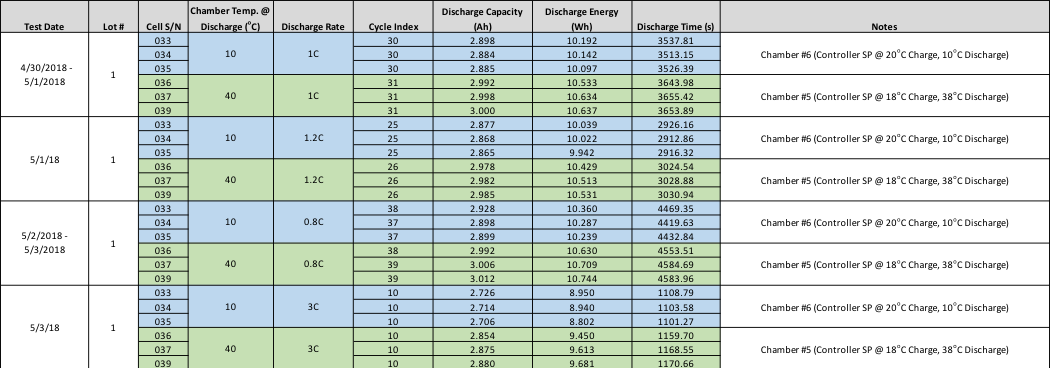
\includegraphics[width=1.0\textwidth]{figures/Test2Summary.png}
	\caption{Test 2 Summary}
	\label{fig:Test2Summary}
\end{figure}

\begin{figure}[!htb]
	\centering
	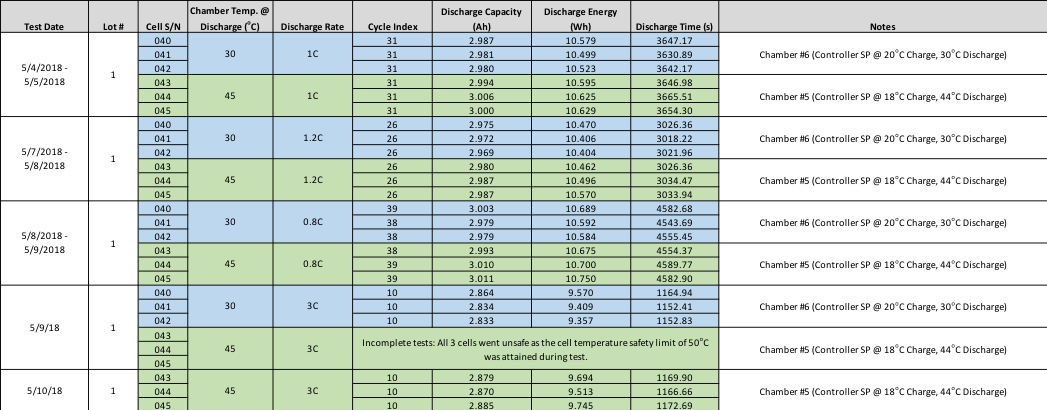
\includegraphics[width=1.0\textwidth]{figures/Test3Summary.png}
	\caption{Test 3 Summary}
	\label{fig:Test3Summary}
\end{figure}

\begin{figure}[!htb]
	\centering
	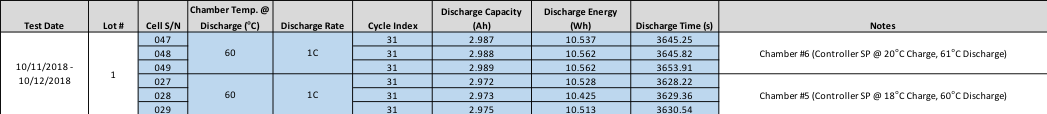
\includegraphics[width=1.0\textwidth]{figures/Test4Summary.png}
	\caption{Test 4 Summary}
	\label{fig:Test4Summary}
\end{figure}

\begin{figure}[!htb]
	\centering
	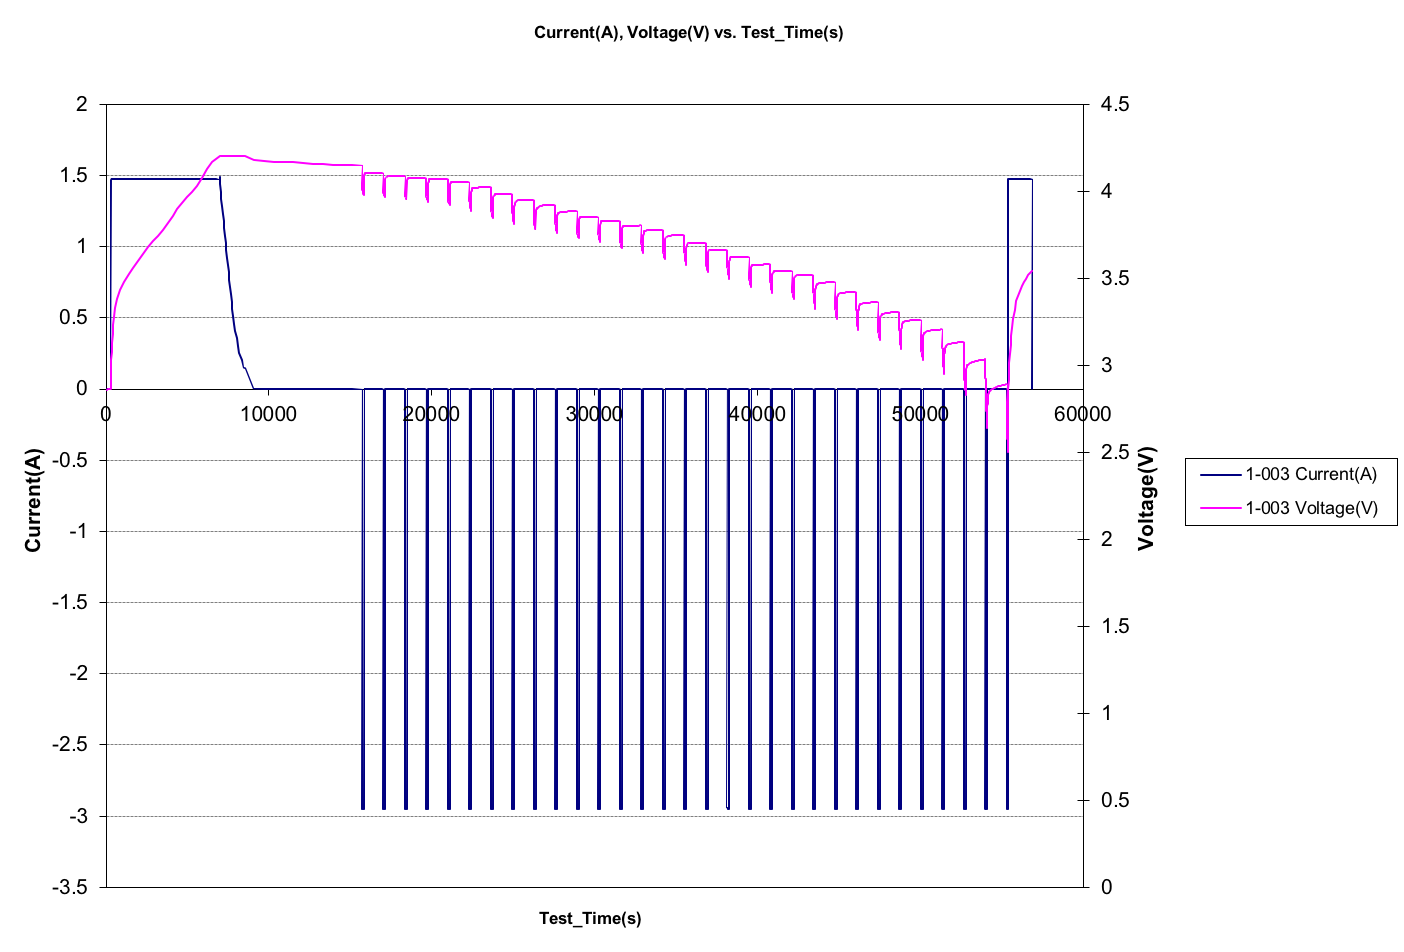
\includegraphics[width=1.0\textwidth]{figures/SampleTest.png}
	\caption{Test 4 Summary}
	\label{fig:Test4Summary}
\end{figure}

\end{document}

% - Release $Name:  $ -

\begin{comment}

\section{Pre/Post Flight Cooling}

X-57 mod II pre-flight CONOPS require that the battery be cooled from an initial state of 60$^\circ$C down to 10$^\circ$C in situ, as removal from the vehicle between test flights is impractical.  A 24-ton commercial aviation air conditioning unit (ACU) was selected for this task.  While dramatically oversized for a light aircraft, the ACU effectiveness will be constrained by the poor convective interface at the battery modules. A range of cooling scenarios were considered, differing in their effective ACU outlet temperatures and degree of mixing or local (flat plate) forced air speed. 


A preliminary analysis treats the battery and aircraft as lumped capacitance coupled through a weak convection interface. This assumption permits rapid permutation of cabin cooling configurations before committing time and resources to a high-fidelity model.  Within the model, each module is characterized by its bulk properties (mass, specific heat), temperature, surface area, and characteristic length. 

These basic battery dimensions and bulk properties contribute to a simplified ‘flat plate’ model of the module surface, where the rate of convective heat transfer between the module and the cabin environment is proportional to surface area (A) and temperature drop across the interface (Tb-T0):

\begin{table}[ht]
\begin{center}
\begin{tabular}{|l|c|c|c|}
\hline
 \multicolumn{1}{|c|}{\textbf{Preconditioning Method}} &
\multicolumn{1}{c|}{\textbf{H per Brick}} & 
\multicolumn{1}{c|}{\textbf{Time to 10$^\circ$C}} &
\multicolumn{1}{c|}{\textbf{Time to 10$^\circ$C}} \\ 
\hline
\rowcolor{LightCyan}
Free Convection  & 0.1-0.3  & 30-140 minutes & 16-80 hrs \\
Good Diffusion + Mixing   & 2 & 5 hrs & 2.5 \\
\rowcolor{LightCyan}
Forced Air Across Modules  & 30 & 0.3 hrs & 0.2\\
\hline
\end{tabular}
\end{center}
\label{tab:batt}
\caption{Cooling Times}
\end{table}

A general outline of preconditioning scenarios was generated form the flat plate battery convection model.  The scenarios represent three typical design points.  The first (and most pessimistic) is a worst case design, where cold air from the ACU is diffused into the vehicle cabin, but at such a low volumetric rate that the modules remain in a free convection state.  The second scenario assumes moderate mixing within the vehicle – either the result of imperfect diffusion from the ACU outlet, or driven by a recirculation fan.  The third scenario represents an ‘advanced’ air cooled design, with purpose-built ductwork directing the cold ACU air into a flat jet impinging on each module interface.  
The effectiveness of the battery preconditioning, as measured by cool-down time (to 10 C) is sensitive to the temperature of the cold air supplied by the ACU, but perhaps more importantly the degree of mixing and forced convection over the modules. 


\begin{figure}[!htb]% order of placement preference: here, top, bottom
	\centering
	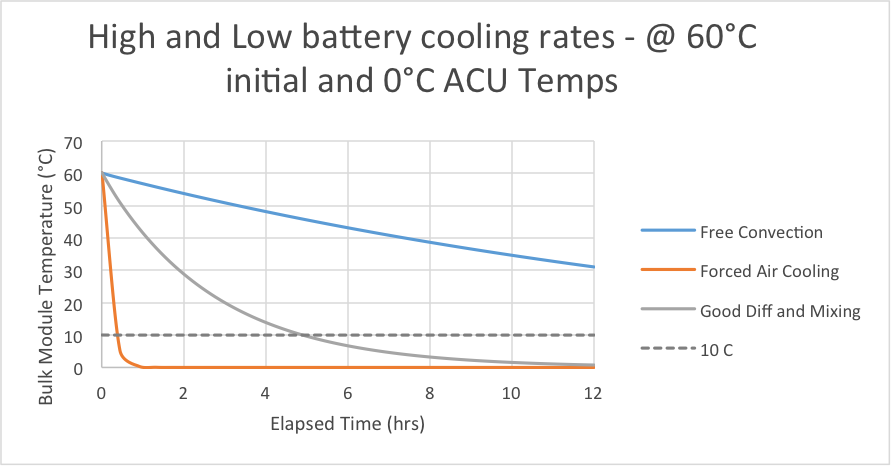
\includegraphics[width=1.0\textwidth]{figures/batt_cooling.png}
	\caption{Battery temperature during ground cooling for multiple scenarios}
	\label{fig:coolingTime}
\end{figure}

\section{In-Flight Thermal Modeling}

% \begin{figure}[!htb]% order of placement preference: here, top, bottom
% 	\centering
% 	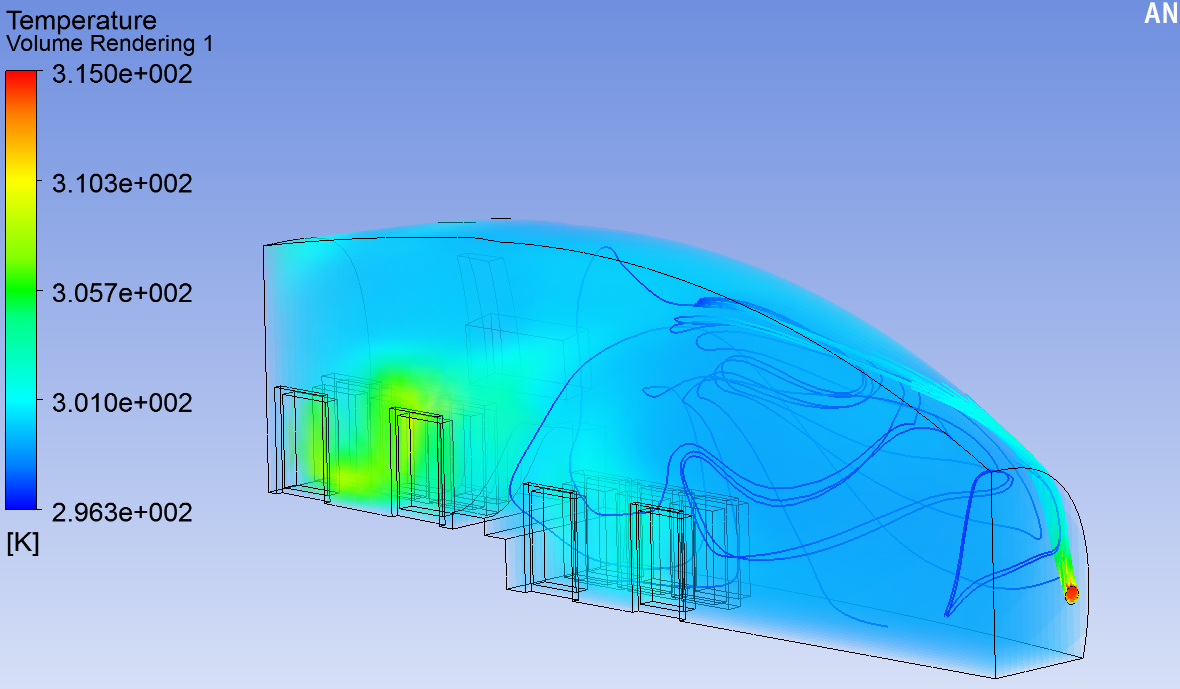
\includegraphics[width=0.75\textwidth]{figures/FuselageAnsys.png}
% 	\caption{Fuselage volume temperature model including air streamlines}
% 	\label{fig:Fuselage}
% \end{figure}

A COMSOL and ANSYS model are being developed to track airflow through the fuselage and determines an ambient air temperature for a separate battery pack COMSOL thermal model.

 \begin{equation}
Q_{conv} = h_{c}*A(t_{b}-t_{0})
\label{eq:Qconv}
\end{equation}


The convective heat transfer coefficient $h_c$ varies depending on the cooling scenario. For air-cooled configurations, it is on the order of $~1 \frac{W}{m^{2} -^{\circ} C}$ for stagnant conditions (free convection) and as high as 450 $\frac{W}{m^{2} -^{\circ} C}$ for forced-air.  Higher $h_c$ values can be computed from the characteristic surface average Nusselt number, Nu: 
 
 \begin{equation}
Nu_{LC} = 0.37*Re_{Lc}^{0.8}*Pr^{0.33}
\label{eq:Nu}
\end{equation}


Where $Re_{Lc}$ is the flat plate Reynolds number, and Pr is the Prandtl number of the surrounding air. The flat plate method is selected because each module ‘brick’ assembly (corresponding to ~1/2 of a module’s cells and support structure) is effectively isolated from its partner. The largest free surface is assumed to account for the majority of convective heat transfer to the vehicle interior. For the mod II vehicle’s battery, each convection surface 

\end{comment}